\chapter{Establishment of laboratory methods and analytical tools to assess genome-wide chromatin accessibility in clinical samples}
\chaptermark{Establishment of methods to assess genome-wide chromatin accessibility}
\label{ch:Results1}


%%%%%%%%%%%%%%%%%%%%%%%%%%%%%%%%%%%%%%%%%%%%%%%%%%
\section{Introduction}
\subsection*{Previous and current methods to identify the accessible genome in cells and tissues}

\subsection*{Implementation of ATAC-seq to define the chromatin landscape}

\subsection*{Technical limitations and recent advances in optimisation}
https://www.ncbi.nlm.nih.gov/pmc/articles/PMC4473780/

Talk about ATAC being more variable, a native chromatin accessibility assessment without cross-linking. Role of transposase ability in accessing the chromatin, debri and DNA from dead cells adding noise

Paper to justify peak calling: A comparison of peak callers used for DNase-Seq data.

New ATAC but also explanations of the limitations: Characterization of chromatin accessibility with a transposome hypersensitive sites sequencing (THS-seq) assay

\subsection*{Challenges of working with clinical samples}

%%%%%%%%%%%%%%%%%%%%%%%%%%%%%%%%%%%%%%%%%%%%%%%%%%
\section{Results}
%

\subsection{Establishment of an ATAC-seq data analysis pipeline based on current knowledge}
When the first ATAC-seq publication \parencite{Buenrostro2013} appeared, there were not well established protocols for the complete processing of the data. Since then, several publications have used ATAC-seq and modifications of this protocol together with a wide range of data analysis strategies to answer different biological questions (Table \ref{tab:ATAC_comparative_methods}).
There are several limiting aspects in the process of analysing ATAC-seq data, including QC assessment, peak calling/filtering and differential analysis of chromatin accessibility regions between groups. Using the current knowledge in the field as well as on my own analysis, I agreed on the most appropriate criteria and parameters to implement in our in-house pipeline. For this purpose, I used ATAC data generated with the original protocol \parencite{Buenrostro2013} in paired CD14$^+$ monocytes and CD4$^+$ total T cells from the same three healthy individuals, all of them downsamples to 30 million of reads, in order to facilitate the comparison across all of them.


%
\begin{landscape}
\begin{center}
\begin{longtable}[ht]{p{.15\textheight} p{.40\textheight} p{.40\textheight} p{.40\textheight}}
\caption{Summary table of ATAC-seq methodology analysis for peak calling, filtering and differential analysis.\textbf{.}}
\label{tab:ATAC_comparative_methods} \\
\toprule
\textbf{Publication} & \textbf{Peak calling and filtering} & \textbf{Master list} & \textbf{Differential analysis} \\
\midrule
\midrule
Corces \textit{et al.}, 2016 & MACS2 (-nomodel), peak summit extension $+/-$250bp, rank summits by pval & Maximally significant non-overlapping peaks. & Quantile normalisation and unsupervised hierarchical clustering. \\

\midrule
ENCODE  & MACS2 -nomodel, pairwise IDR analysis, filtering IDR$<$10\% & Choosing longest pairwise IDR filtered list or only peaks present in the two samples pseudoreplicates. & NA \\
              
\midrule
Turner \textit{et al.}, 2018 	& MACS2 (-nomodel --q 0.01) & Merging all filtered called peaks from the different cell types. & \texti{De novo}:DiffReps with fragment size 50bp. \\                             
																																										
\midrule
Alasoo \textit{et al.}, 2018 & MACS2 (-nomodel -shift -25 -extsize 50 --q 0.0 &	Union of peaks from all conditions present in at leats in three samples of the same condition. & Peak based: TMM normalisation and lima voom (FDR$<$0.01).\\ 

\midrule
Qu \textit{et al.}, 2017 & ZINBA PP$>$0.99. & Merging of filtered peaks from each individual sample. & Quantile normalisation and peak based in house Pearson correlation method. \\							

\midrule
Rendeiro \textit{et al.} 2016 & MACS2 (-nomodel -extsize 147)	& Merge of peaks from all samples in an iterative process including permutations & Peak based: quantile normalisation and Fisher exact text (FDR$<$0.05). \\

\midrule
Scharer\textit{et al.} 2016 & HOMER (-style dnase) & Merge of all overlapping peaks between all samples using HOMER mergePeaks & Peak based: TMM normalisation and edgeR package (FDR$<$0.05). \\														   
\bottomrule
\medskip
\end{longtable}
\end{center}
\end{landscape}

%\clearpage



\subsubsection{Sample quality control}
Regarding QC measurements, the variability in performance of the methodology, particularly ATAC-seq and Fast-ATAC, has required to agree on appropriate parameters to determine the quality of the samples before proceeding with downstream differential analysis. After reviewing the different read-outs implemented across different publications, I have identified the most informative ones showing supporting correlation between them.

Firstly, I analysed the fragment size distribution for each of the samples in order to determine if they recapitulated the expected nucleosome periodicity every $\sim$200bp (Figure \ref{fig:QC_ATAC}a). All the samples showed periodicity up to 600bp, clearly distinguishing chromatin organisation into mono-, di- and tri-nucleosomes. The relative intensity of nucleosome-free DNA fragments ($<$200pb) compared to nucleosome-bound DNA was greater for some of the samples (e.g CTL1 CD4$^+$ and CD14$^+$) and similar or lower for others (e.g CTL3 CD4$^+$ and CD14$^+$). Nucleosome-free fragments ($<$147bp) are also clearly distinguished in all of the samples, meeting the ENCODE QC recommendations \parencite{ENCODE}.

Another QC measurement was based on the enrichment over a random background of ATAC-seq reads across all the TSS for the identified for Ensemble genes (Figure \ref{fig:QC_ATAC}b). It is well established that nucleosome repositioning and an increase of chromatin accessibility take place at TSS to allow formation of the transcriptional machinery and initiation of transcription. Fold-enrichment signals ranged between 5-7 for the CD4$^+$ samples and they were much higher(between 17-20) for the CD4$^+$ samples. The lower sample quality of the CD4$^+$compared to CD14$^+$ shown by the TSS signal were recapitulated by the ATAC-seq genome browser density at the promoter of the constitutively expressed gene \textit{GAPDH} (Figure \ref{fig:QC_ATAC}c). 
	
As part of the QC assessment I looked at the percentage of mitochondrial reads and the fraction of reads in peaks (FRiP)(Table \ref{tab:ATAC_MT_fraction_reads_in_peaks}). 

\begin{table}[htbp]
%\setlength{\tabcolsep}{20pt} only to stretch the columns if you want
%\renewcommand{\arraystretch}{1.5}
\centering
\begin{tabular}{@{} c c c}
\toprule
\textbf{Sample} & \textbf{\% MT reads} & \textbf{Fraction of reads in peaks} \\
\midrule
\midrule
CTL1 CD4 & 14.9 & 9.8 \\
CTL2 CD4 & 30.5 & 11.2 \\
CTL3 CD4 & 28.8 & 11.6 \\
CTL1 CD14 & 43.3 & 32.2 \\
CTL2 CD14 & 36.8 & 57.0 \\
CTL3 CD14 & 37.6 & 49.9 \\
\bottomrule
\end{tabular}
\medskip %gap
\caption[ATAC-seq percentage of MT reads and fraction of reads in called peaks]{\textbf{}}
\label{tab:ATAC_MT_fraction_reads_in_peaks}
\end{table}
\bigskip %bigger space


Positive correlation between the TSS fold-change enrichment and FRiP was observed, being both appropriate inter-dependent QC measures to evaluate sample noise (Figure \ref{fig:QC_ATAC}d). Regarding the cut-off values, Alsoo \textit{et al.}, 2018 and, recently, ENCODE have recommended minimum FRiP between 10-20\% and TSS between 6-10. ENCODE has prioritised the use of TSS over FRiP as the measurement to determine the noise in the sample \parencite{ENCODE}. The mitochondrial content ranged between 14.9-43.3\% and, alike FRiP and TSS, it was higher in CD4$^+$ than in CD4$^+$ and was cell type dependent and not directly related with any of the other QC measurements.



\begin{figure}[htbp]
\centering
\begin{subfigure}{0.45\textwidth}
\centering
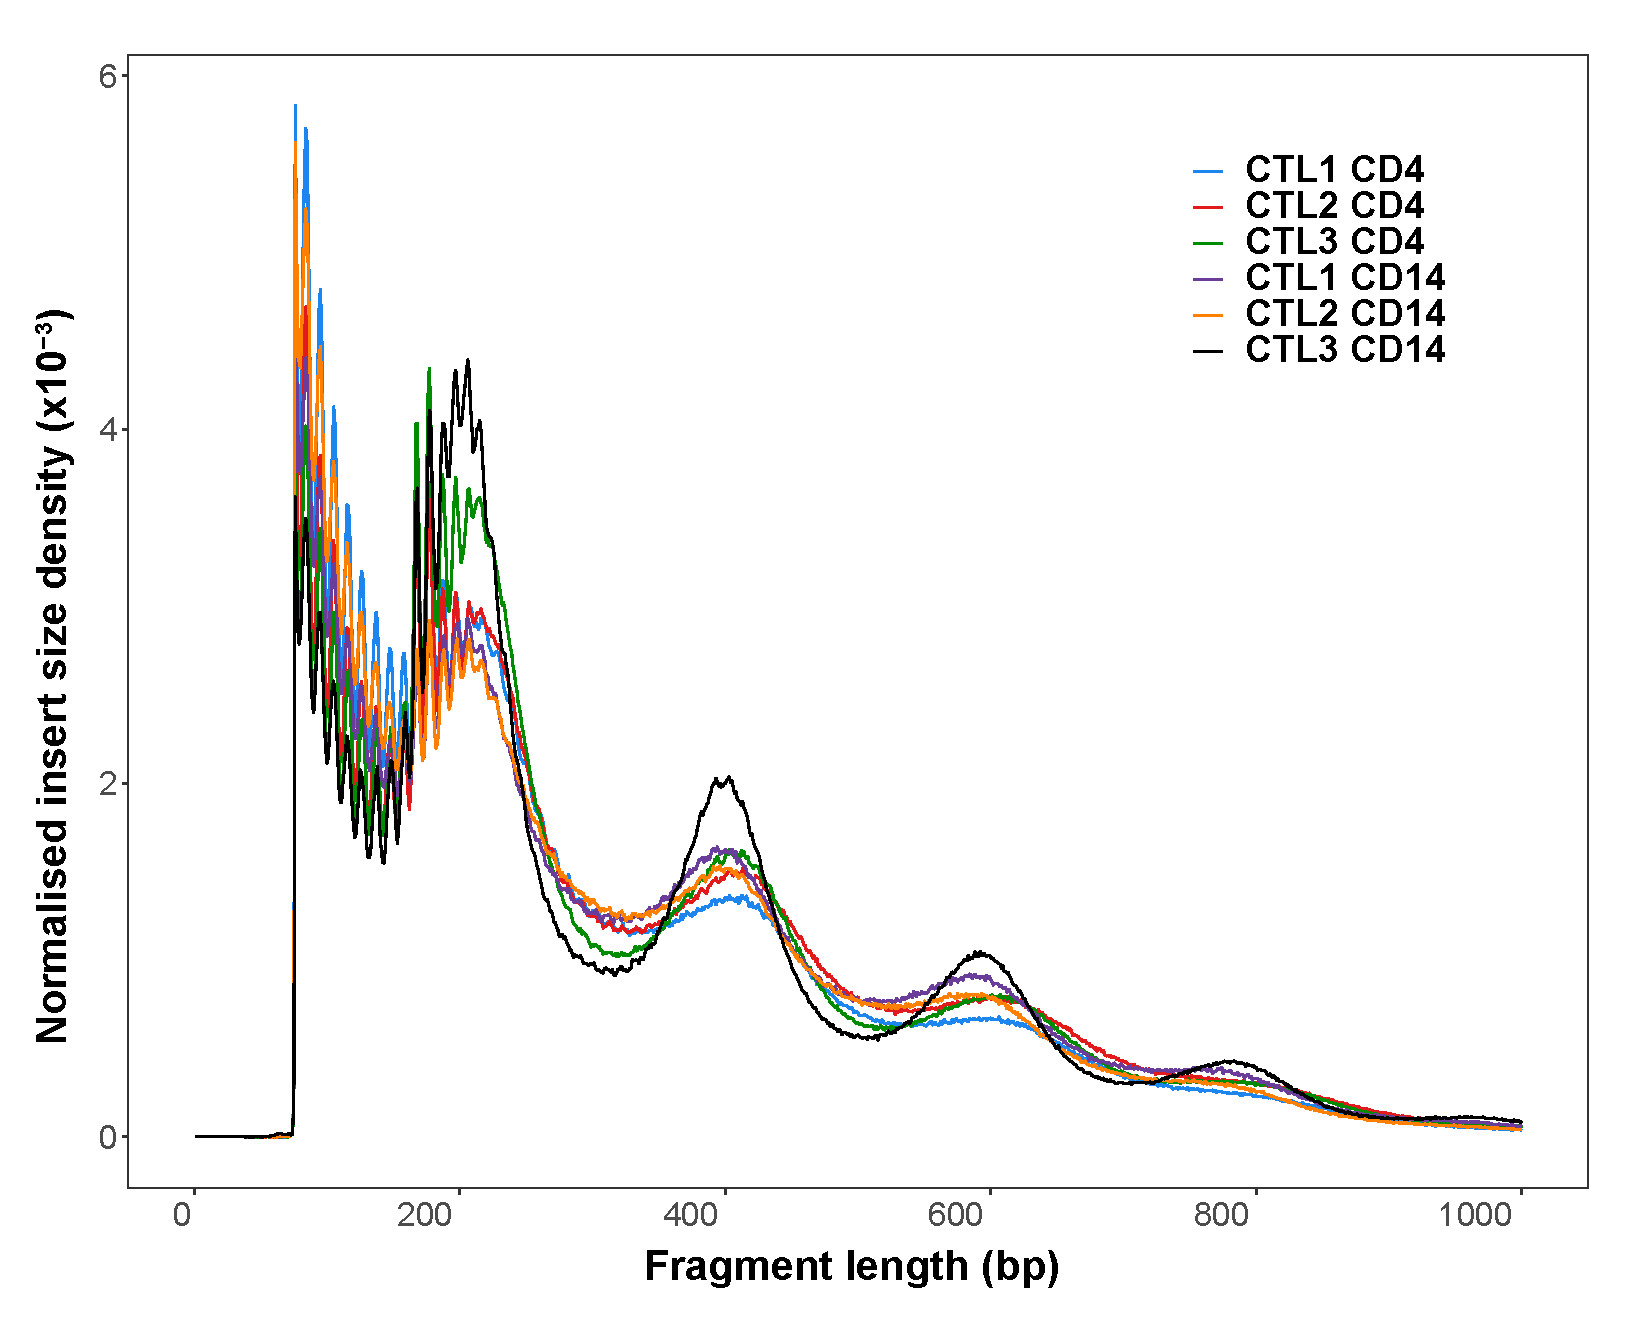
\includegraphics[height=8cm,width=\textwidth]{./Results1/pdfs/ATAC_Core_fresh_CD4_CD14_frag_size_distribution}
\caption{\textbf{}}
% The percentage sign indicated that the other subfig goes side by side
\end{subfigure}%
\begin{subfigure}{0.45\textwidth}
\centering
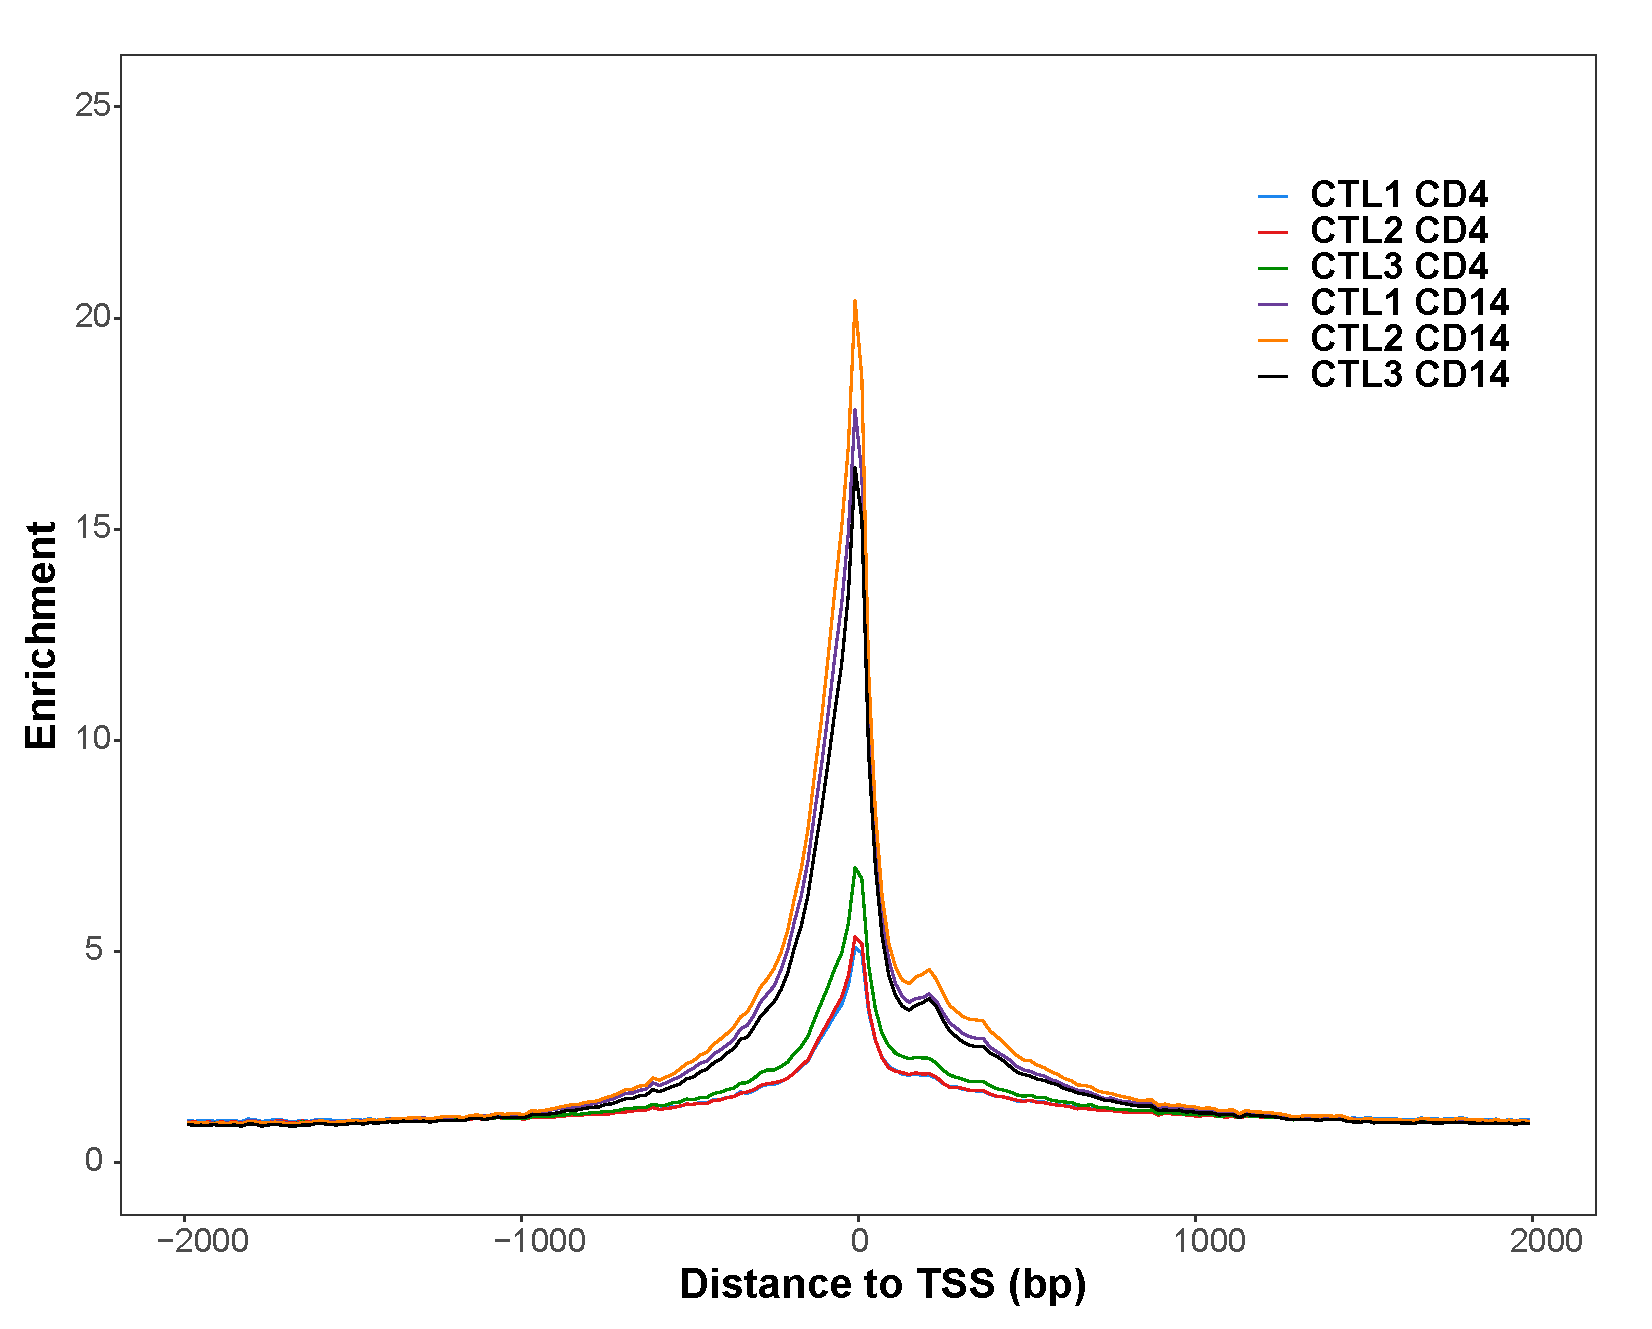
\includegraphics[height=8cm,width=\textwidth]{./Results1/pdfs/TSS_enrichment_Core_fresh_CD4_CD14}
\caption{\textbf{}}
\end{subfigure} \\
\hfill
\begin{subfigure}{0.45\textwidth}
\centering
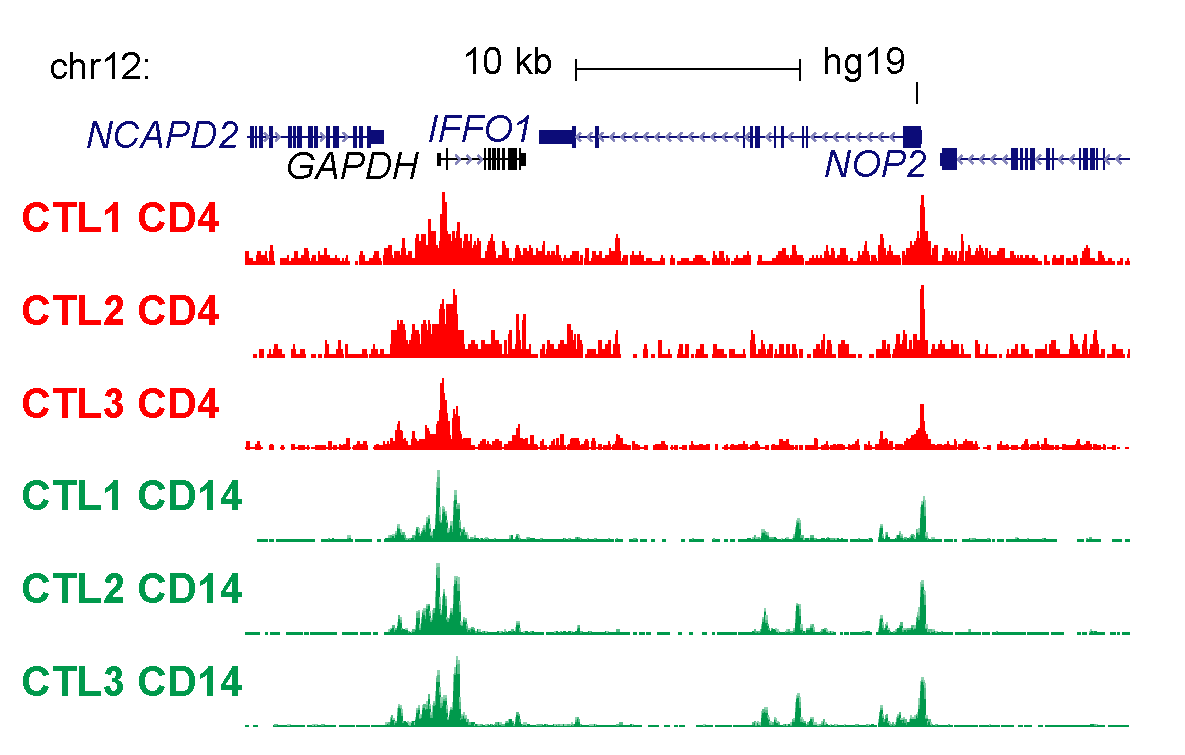
\includegraphics[height=8cm,width=\textwidth]{./Results1/pdfs/ATAC_Core_CD4_CD14_fresh_GAPDH}
\caption{\textbf{}} % to add text to the figure name
\end{subfigure}%
\begin{subfigure}{0.45\textwidth}
\centering
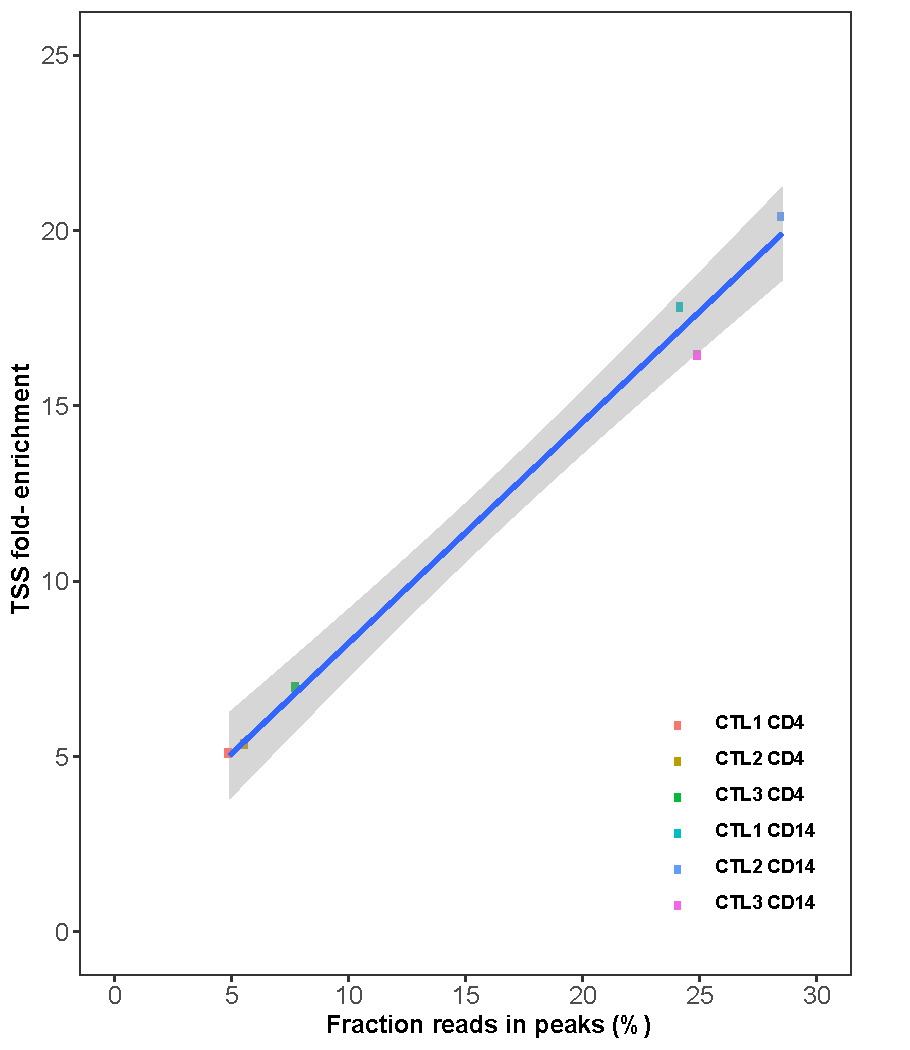
\includegraphics[height=8cm,width=\textwidth]{./Results1/pdfs/ATAC_Core_fresh_CD4_CD14_corr_tss_vs_frac_reads_in_peaks}
\caption{\textbf{}} % to add text to the figure name
\end{subfigure} \\
\hfill
\caption[Measurements for quality control assessment in ATAC-seq samples]{\textbf{} \\
}
\label{fig:QC_ATAC}
\end{figure}
	

\subsubsection{Peak calling and filtering}
As part of the ATAC-seq pipeline implementation, peak calling and the criteria for filtering where another two aspects to determine.
Although different peak callers have been used, most of the publications as well as ENCODE has been using MACS2 as the preferred methodology (Table \ref{tab:ATAC_comparative_methods}). MACS2 has been initially developed for ChIP but it has also been used for DHS and ATAC-seq with disabling the model and agreeing in an extension size (--extsize) and a shift (--shift), which indicate the direction and number of bp for reads to be shifted and the number of bp for them to be extended, respectively. The --extsize should correspond to the average fragment size, which in my libraries is $\sim$200bp and the --shift is set to -100, as it is recommended to be set to -1/2 of the fragment size for chromatin accessibility assays. This parameter could be further optimised but it escapes from the aim of this thesis.

I was interesting in understanding the effect of sequencing depth and the sample quality on the peak calling to have a better control of both variables in the downstream analysis. I performed random read sub-sampling every 5M total reads (from 5M to 30M) followed by peak calling with arbitrary filtering for FDR$<$0.01 in each of the six aforementioned samples. 

Number of reads is dependent of the read depth and sample quality. Lower number of peaks called in CD4 samples compared to CD14, reflecting sample quality effect. However for both set of samples number of called peaks increases with the number of reads and when looking at the increment of number of peaks both reach plateau


\begin{figure}[htbp]
\centering
\begin{subfigure}{0.45\textwidth}
\left
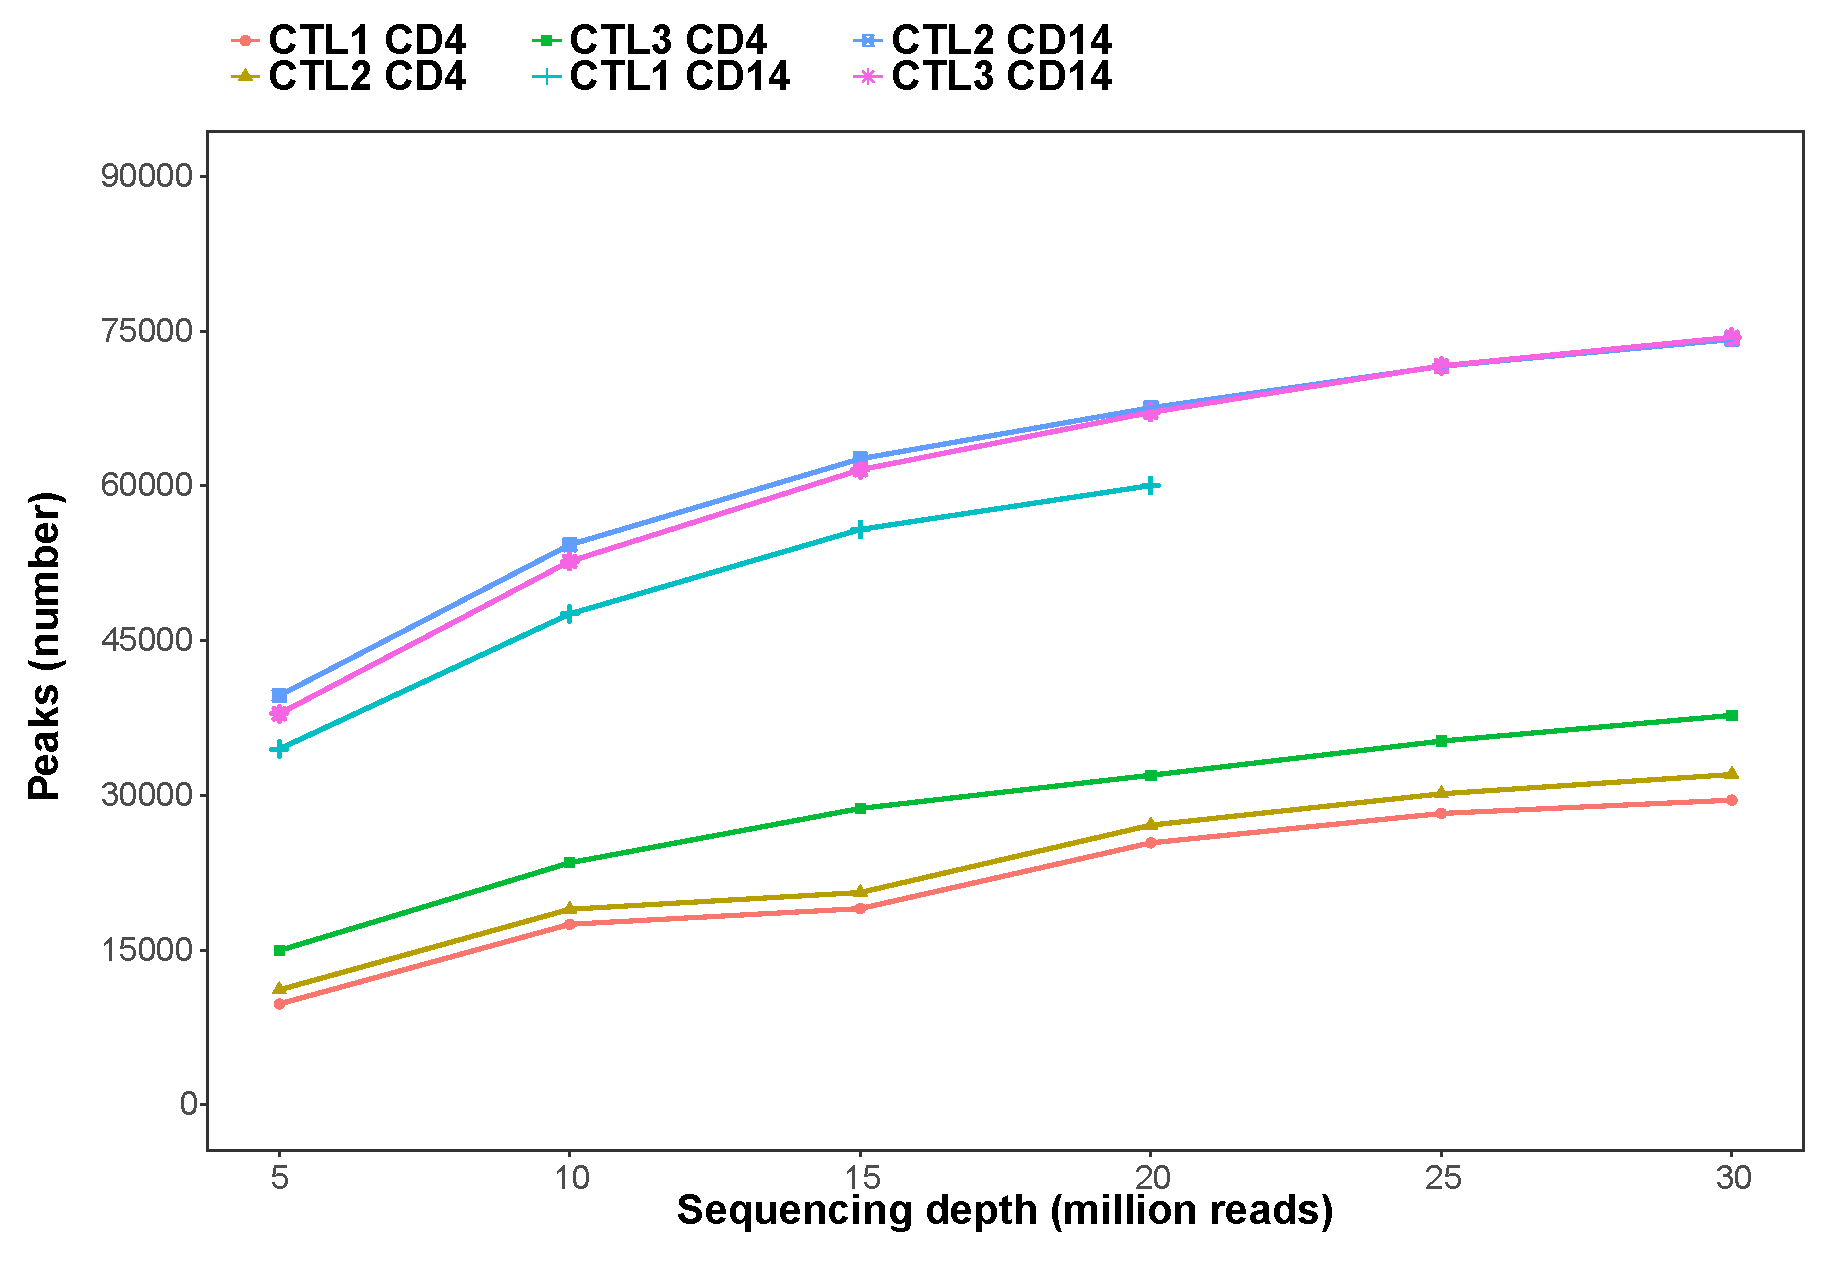
\includegraphics[width=\textwidth]{./Results1/pdfs/ATAC_Core_fresh_CD4_CD14_num_peaks_vs_depth}
\caption{\textbf{}}
% The percentage sign indicated that the other subfig goes side by side
\end{subfigure}%
\begin{subfigure}{0.45\textwidth}
\right
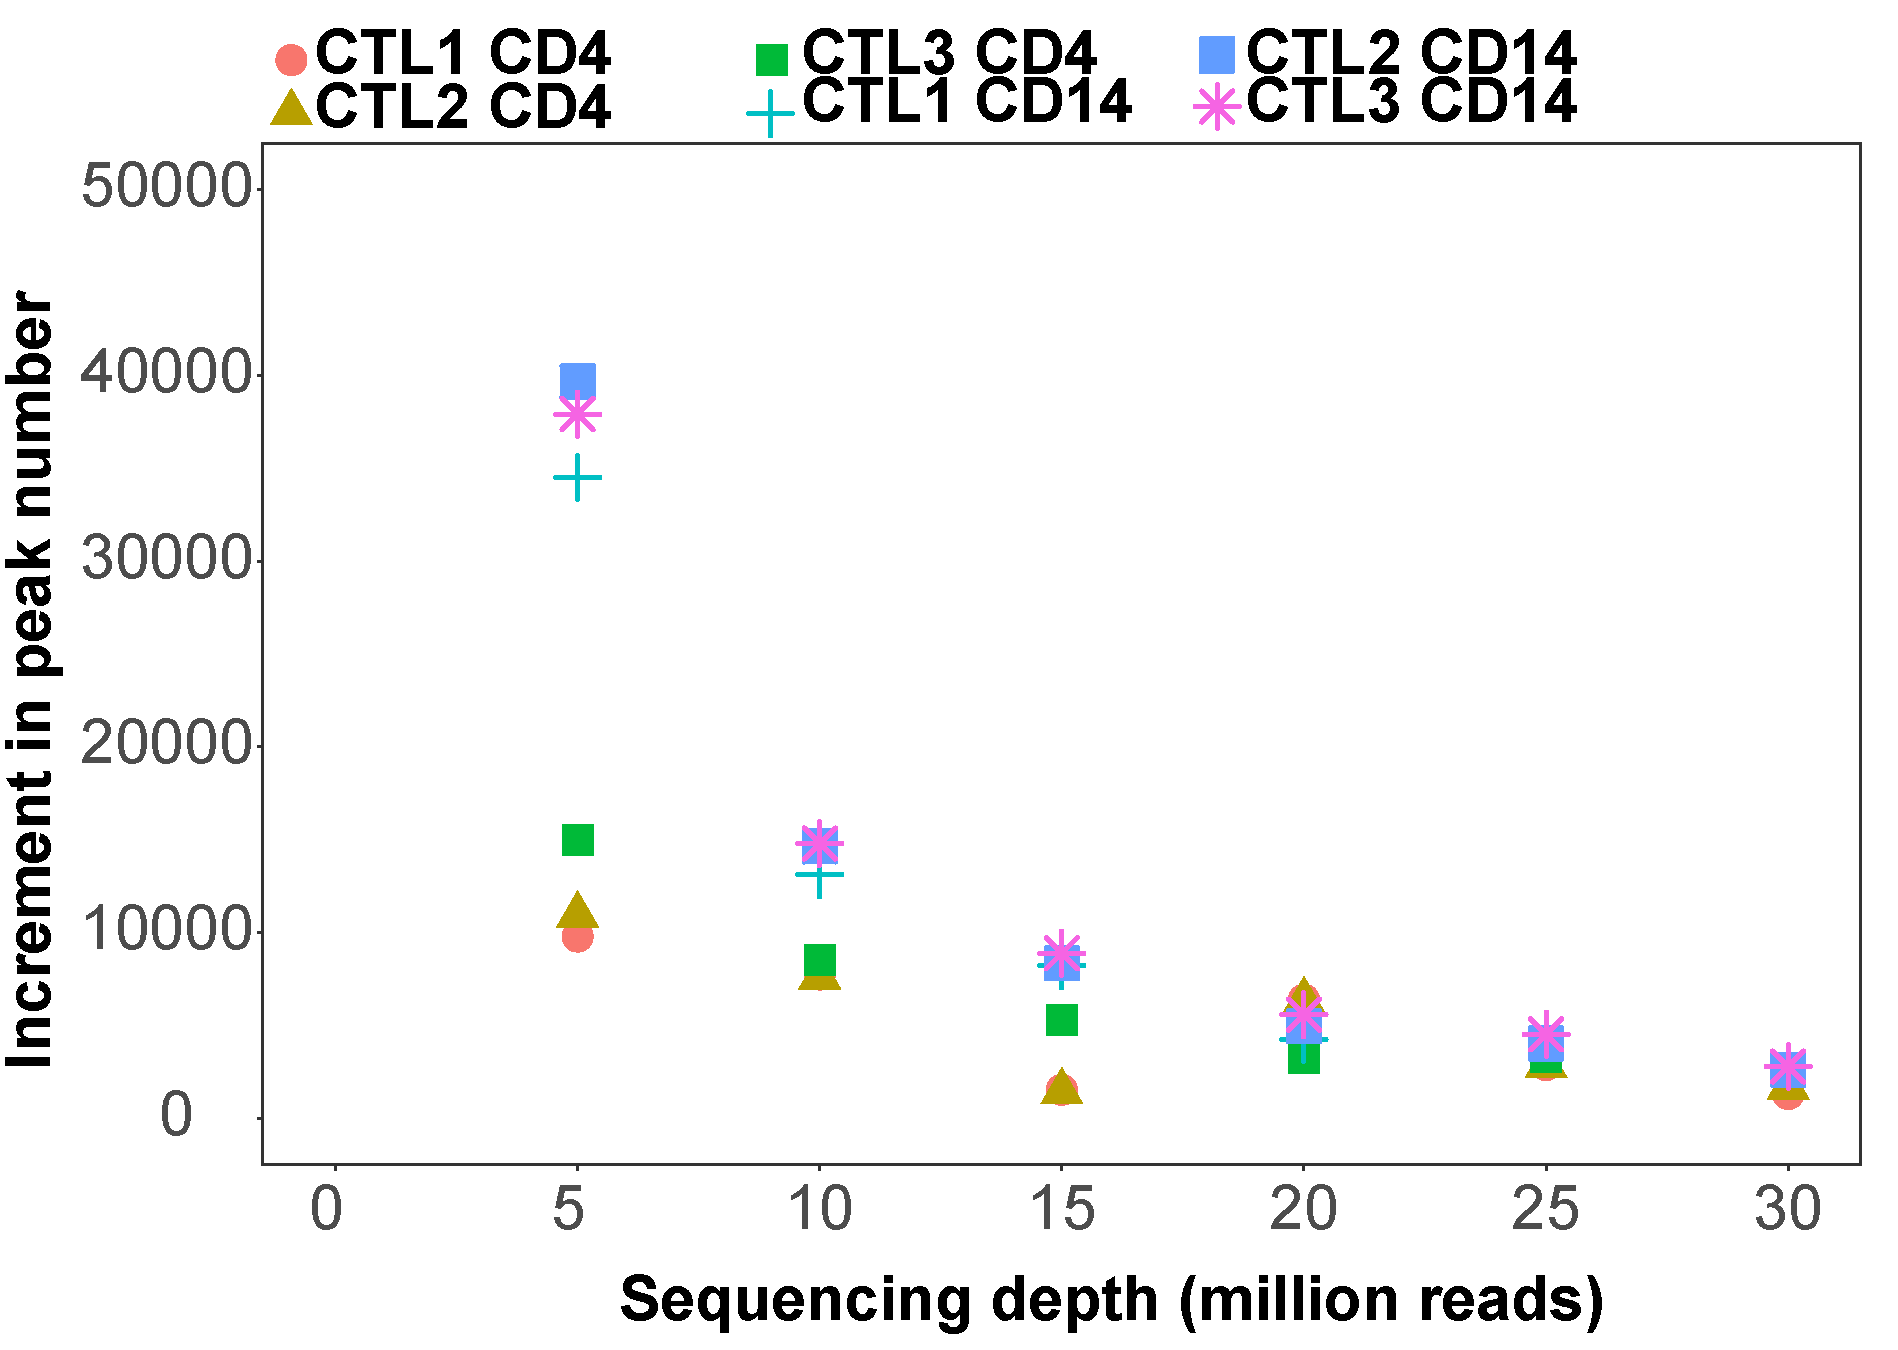
\includegraphics[width=\textwidth]{./Results1/pdfs/ATAC_Core_fresh_CD4_CD14_increment_num_peaks_vs_depth}
\caption{\textbf{}}
\end{subfigure} \\
\begin{subfigure}{0.5\textwidth}
\centering
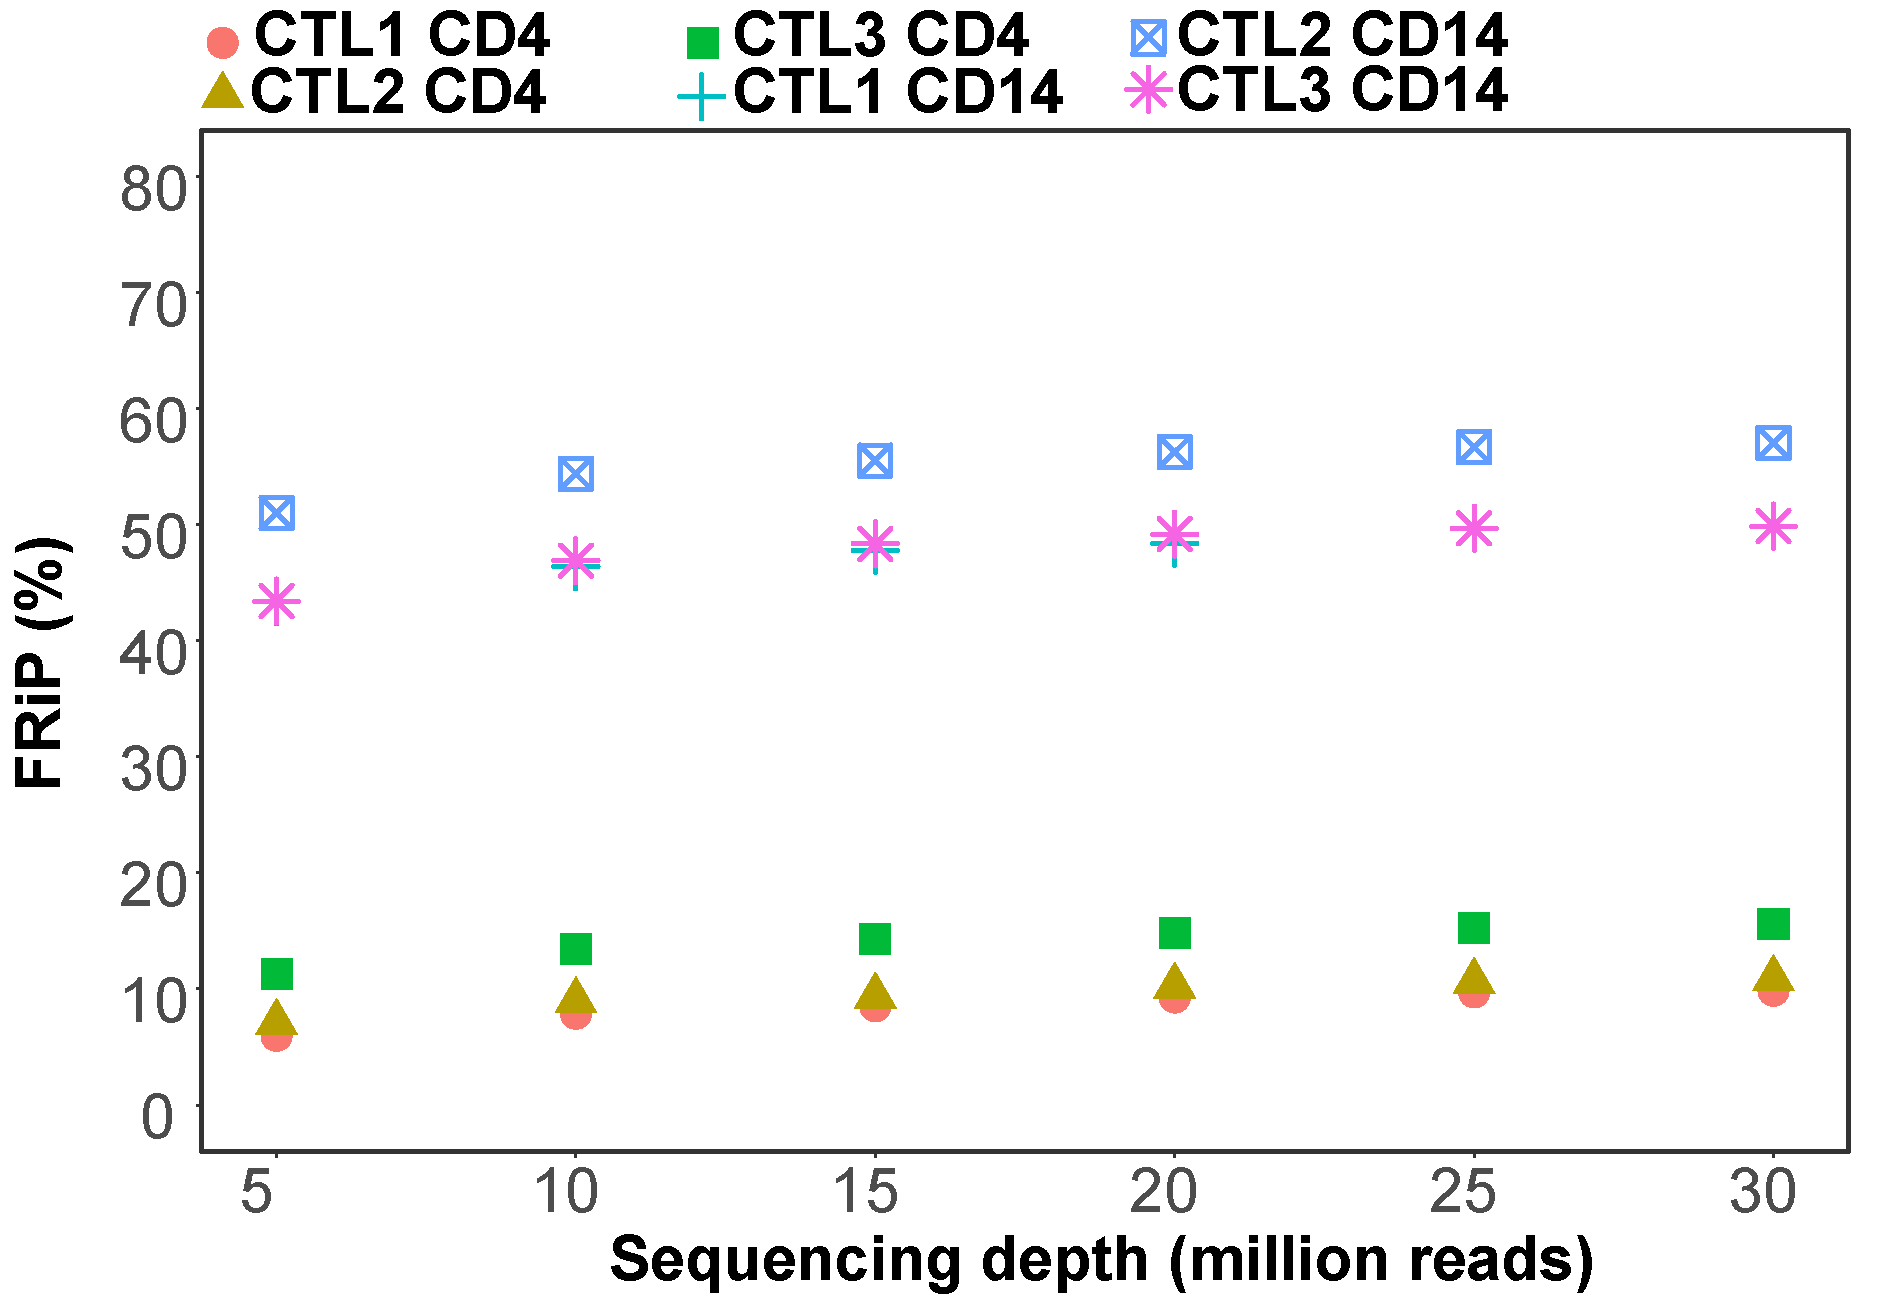
\includegraphics[width=\textwidth]{./Results1/pdfs/ATAC_Core_fresh_CD4_CD14_frac_reads_in_peaks_vs_depth}
\caption{\textbf{}} % to add text to the figure name
\end{subfigure}%
\caption[Peak calling and sequencing depth in ATAC-seq samples]{\textbf{Peak calling at different sequencing depth in ATAC-seq samples} \\
}
\label{fig:Peak_calling_versus_depth_ATAC}
\end{figure} 




\begin{figure}[htbp]
\centering
\begin{subfigure}{0.5\textwidth}
\centering
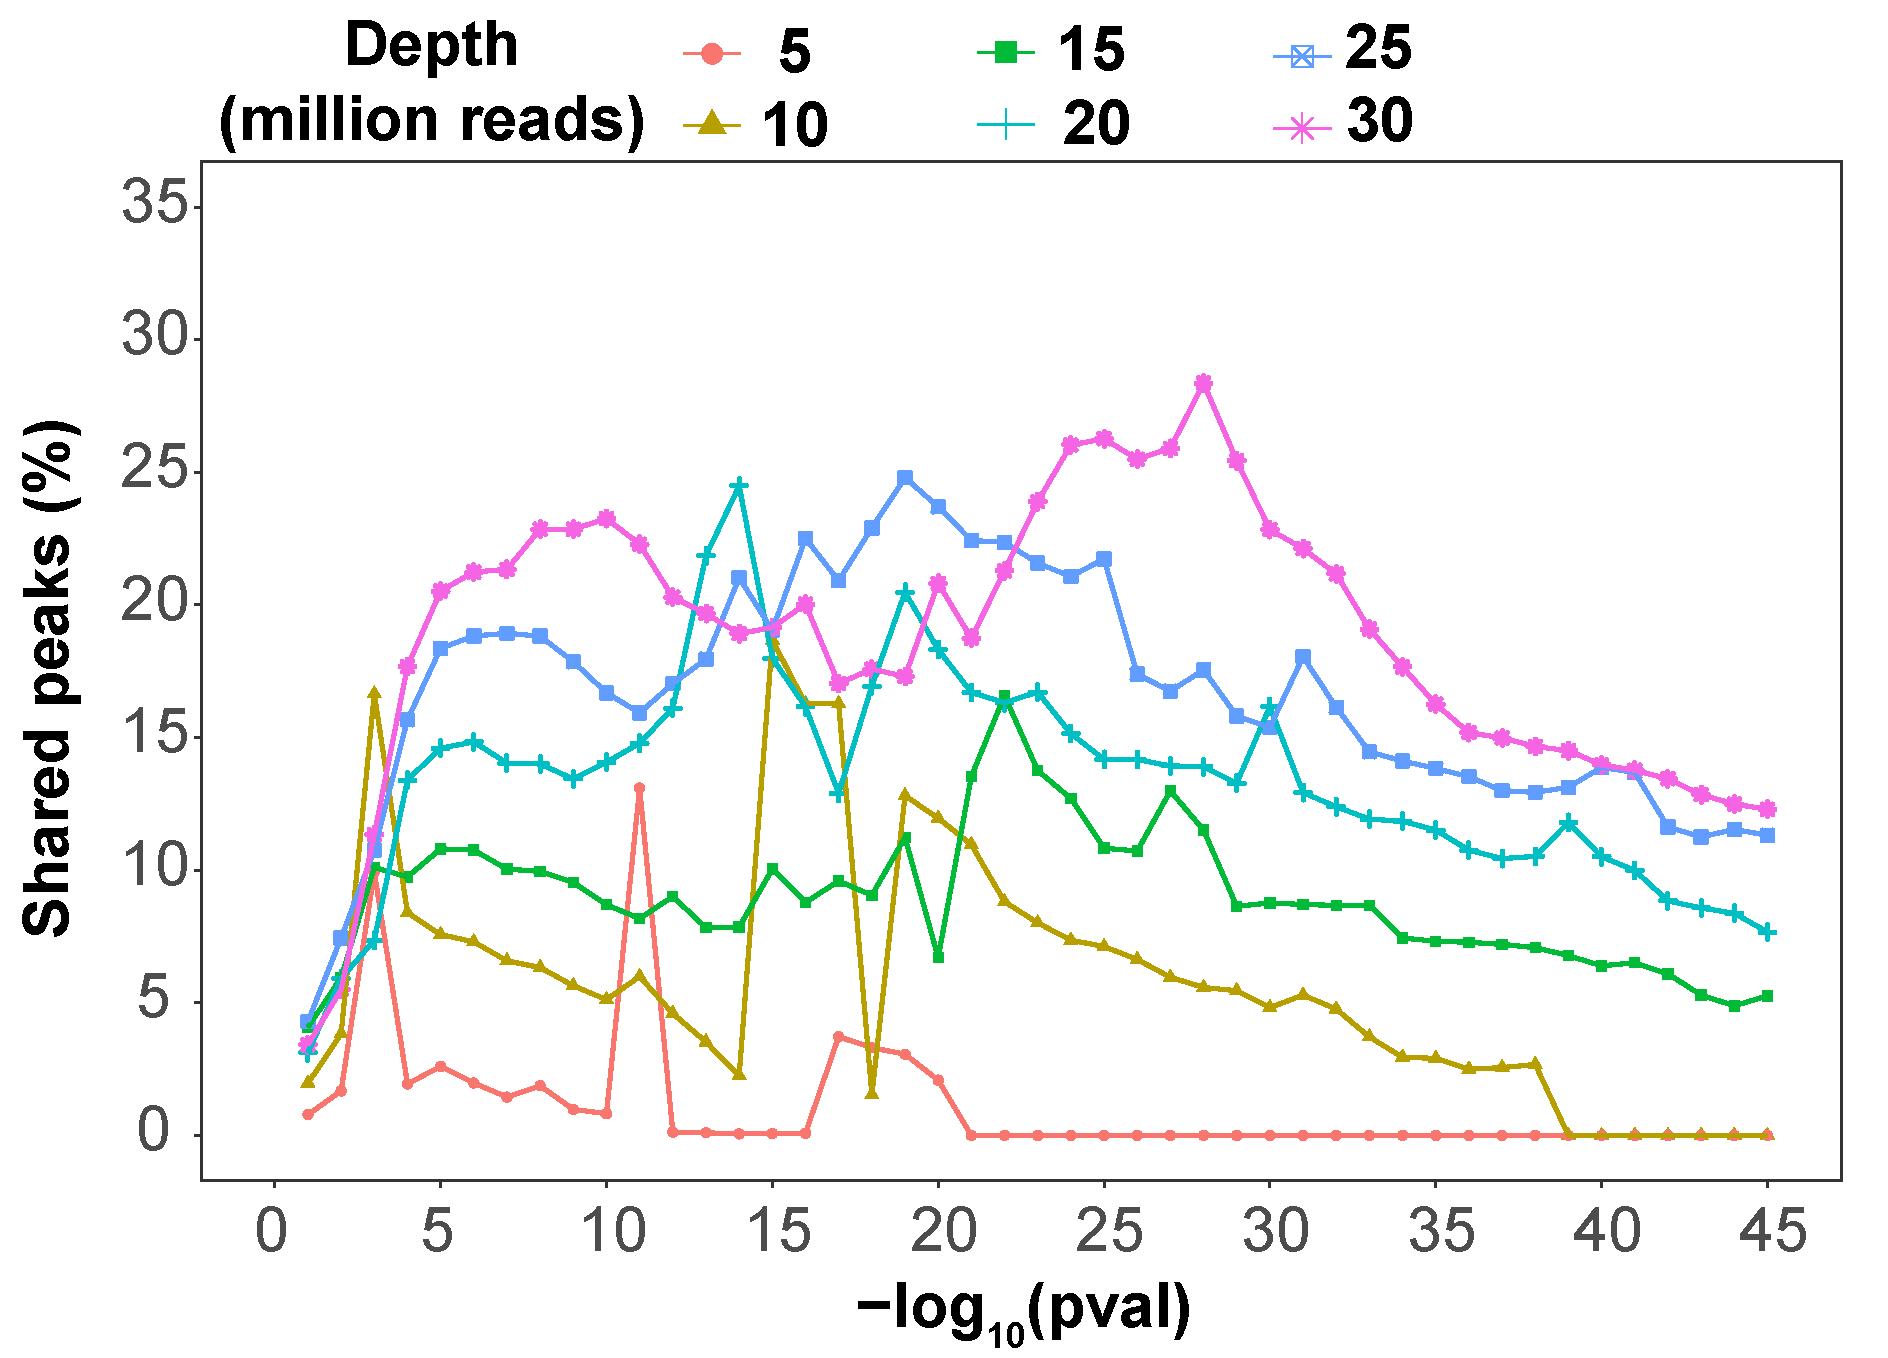
\includegraphics[width=\textwidth]{./Results1/pdfs/ATAC_Core_fresh_CTL2_CD4_shared_peaks_IDR_vs_pval}
\caption{\textbf{}}
% The percentage sign indicated that the other subfig goes side by side
\end{subfigure}%
\begin{subfigure}{0.5\textwidth}
\centering
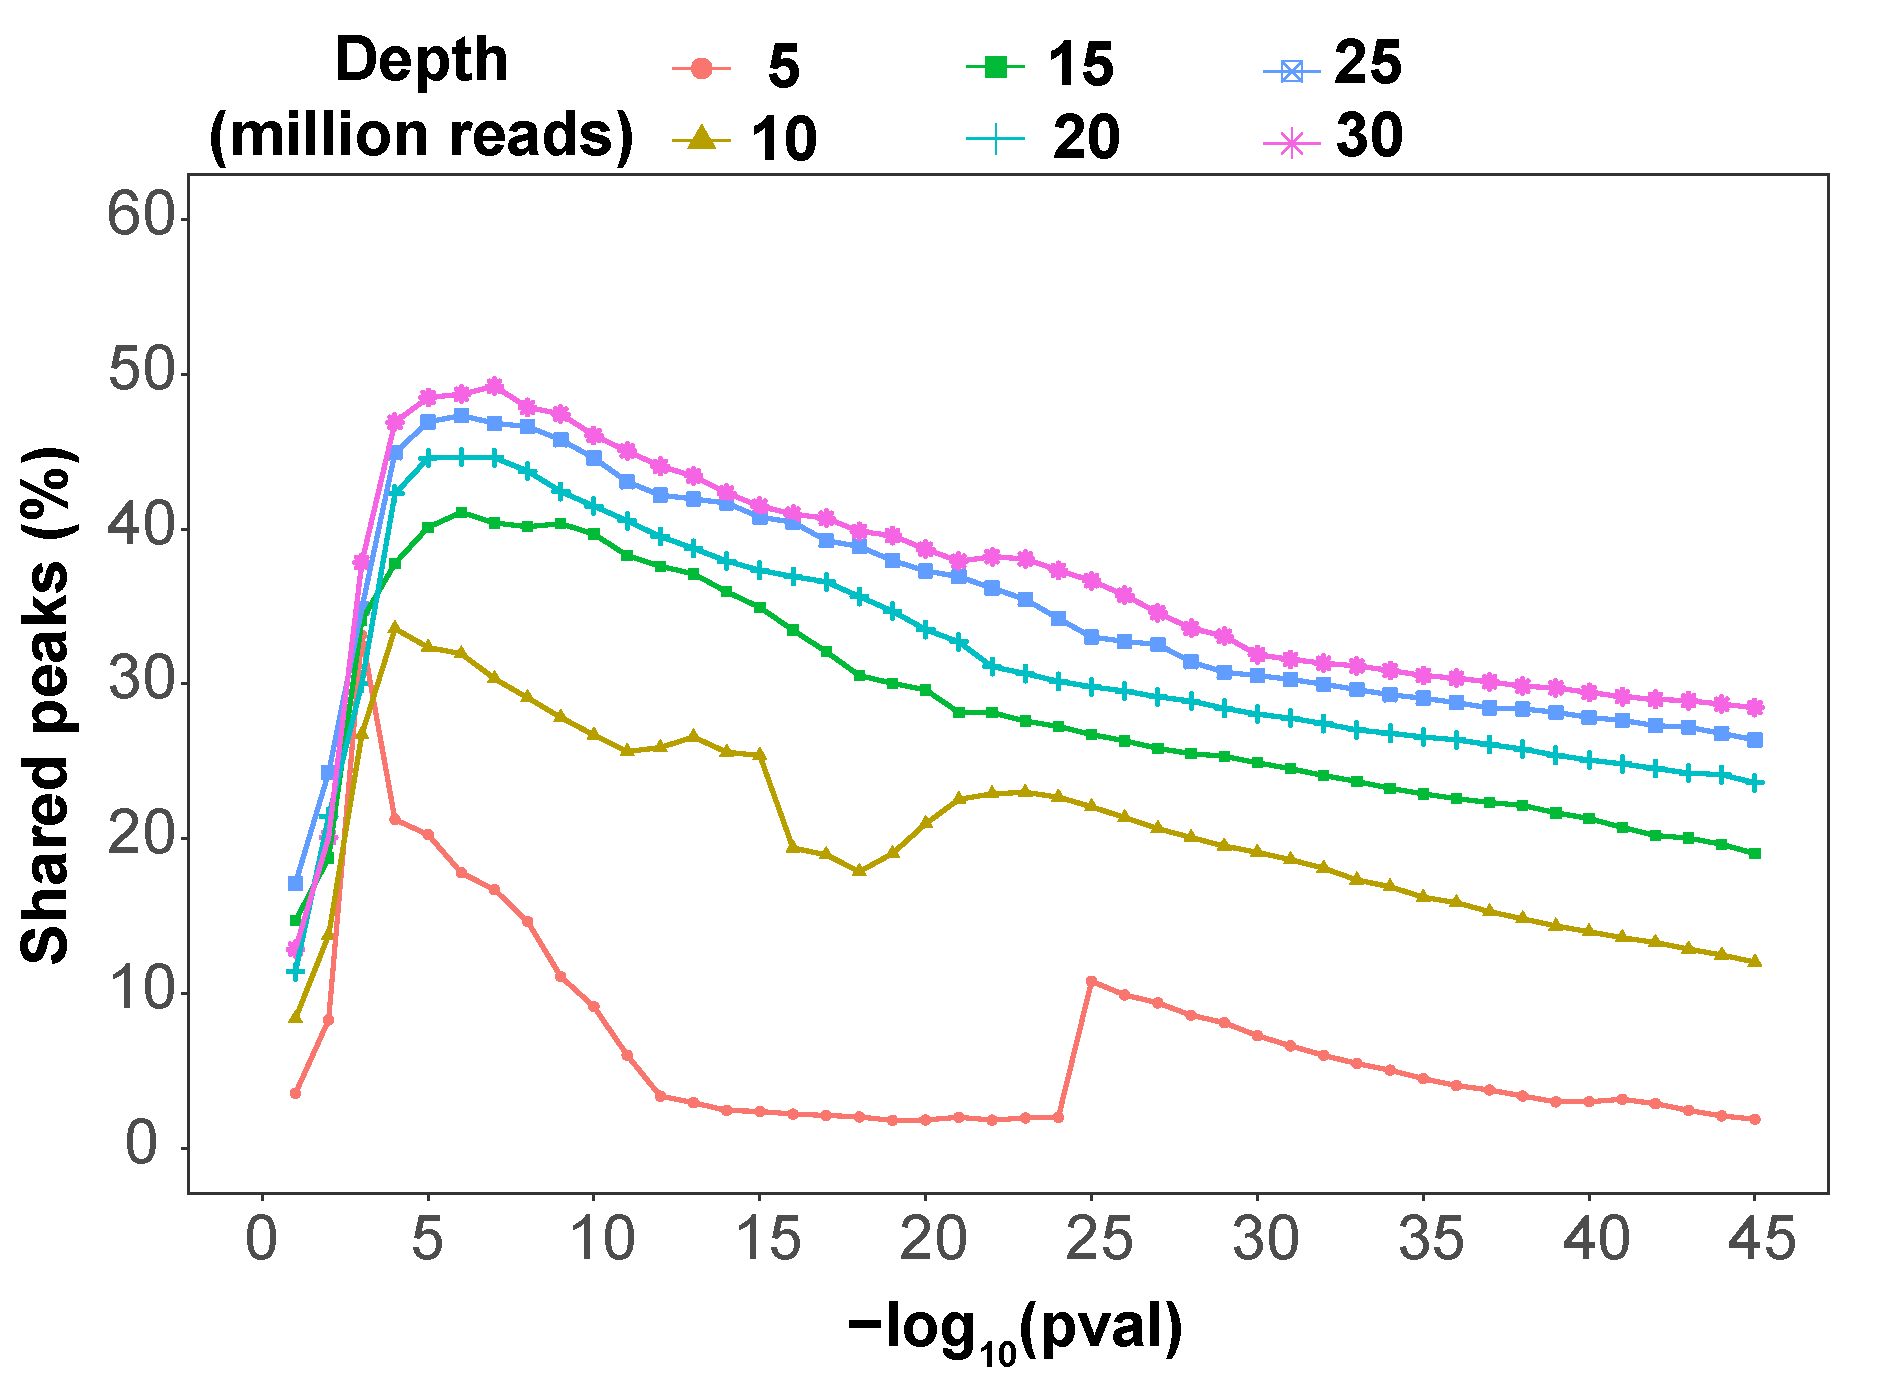
\includegraphics[width=\textwidth]{./Results1/pdfs/ATAC_Core_fresh_CTL2_CD14_shared_peaks_IDR_vs_pval}
\caption{\textbf{}}
\end{subfigure} \\
\begin{subfigure}{0.5\textwidth}
\centering
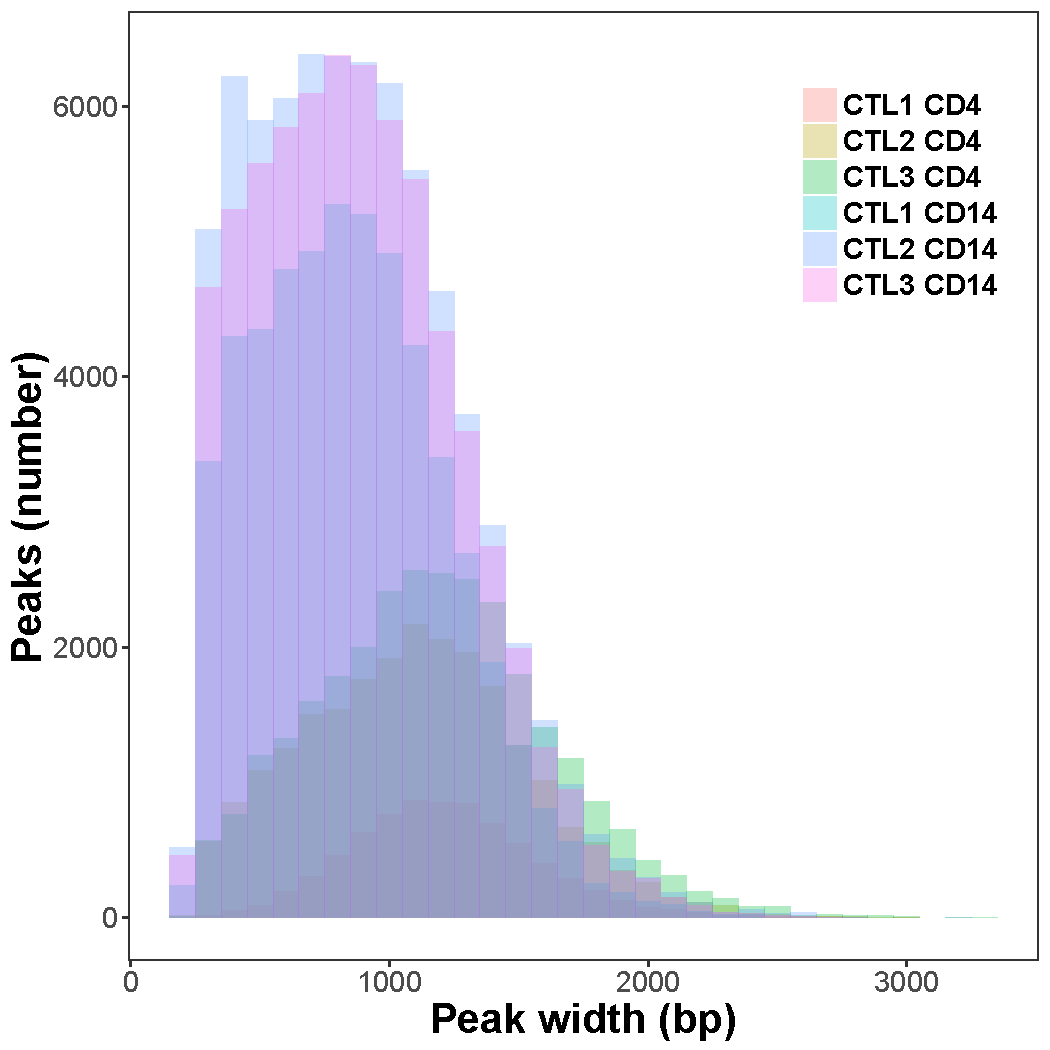
\includegraphics[width=\textwidth]{./Results1/pdfs/peak_width_hist_CD4_CD14_PVAL_IDR_filtered_peaks}
\caption{\textbf{}} % to add text to the figure name
\end{subfigure}%
\caption[Peak calling assessment and IDR filtering in ATAC-seq samples]{\textbf{Peak calling filtering and assessment of width distribution in ATAC-seq samples} \\
}
\label{fig:Peak_calling_IDR_filtering_and_width_ATAC}
\end{figure} 



\subsection{Assessment of ATAC-seq transposition times and comparison with FAST-ATAC protocol in relevant cell types}


\begin{figure}[htbp]
\centering
\begin{subfigure}{0.5\textwidth}
\centering
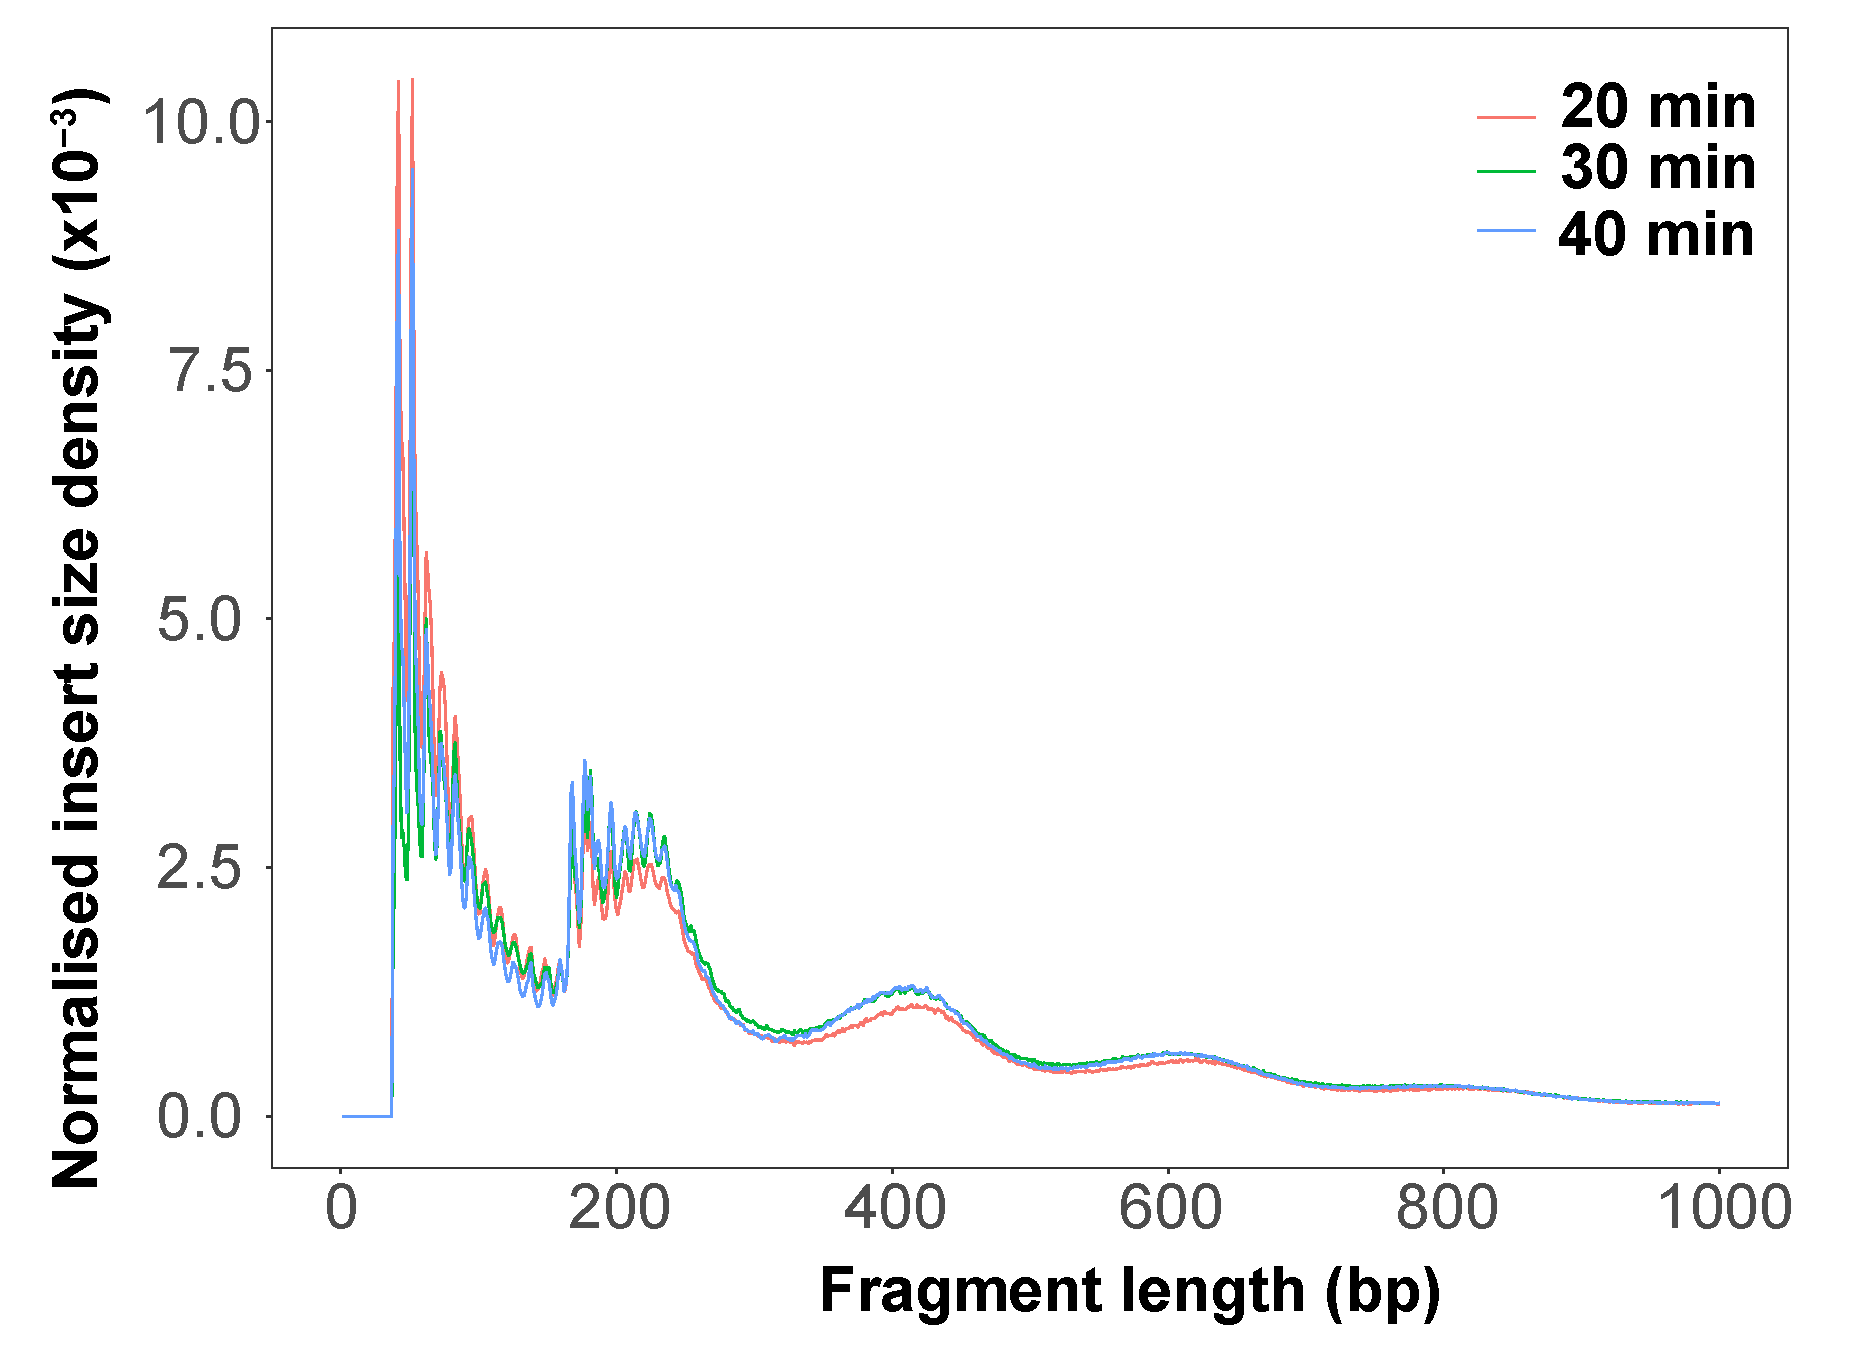
\includegraphics[width=\textwidth]{./Results1/pdfs/ATAC_CD8_fragment_size_distribution_20_30_40min}
\caption{\textbf{}}
% The percentage sign indicated that the other subfig goes side by side
\end{subfigure}
\begin{subfigure}{0.5\textwidth}
\centering
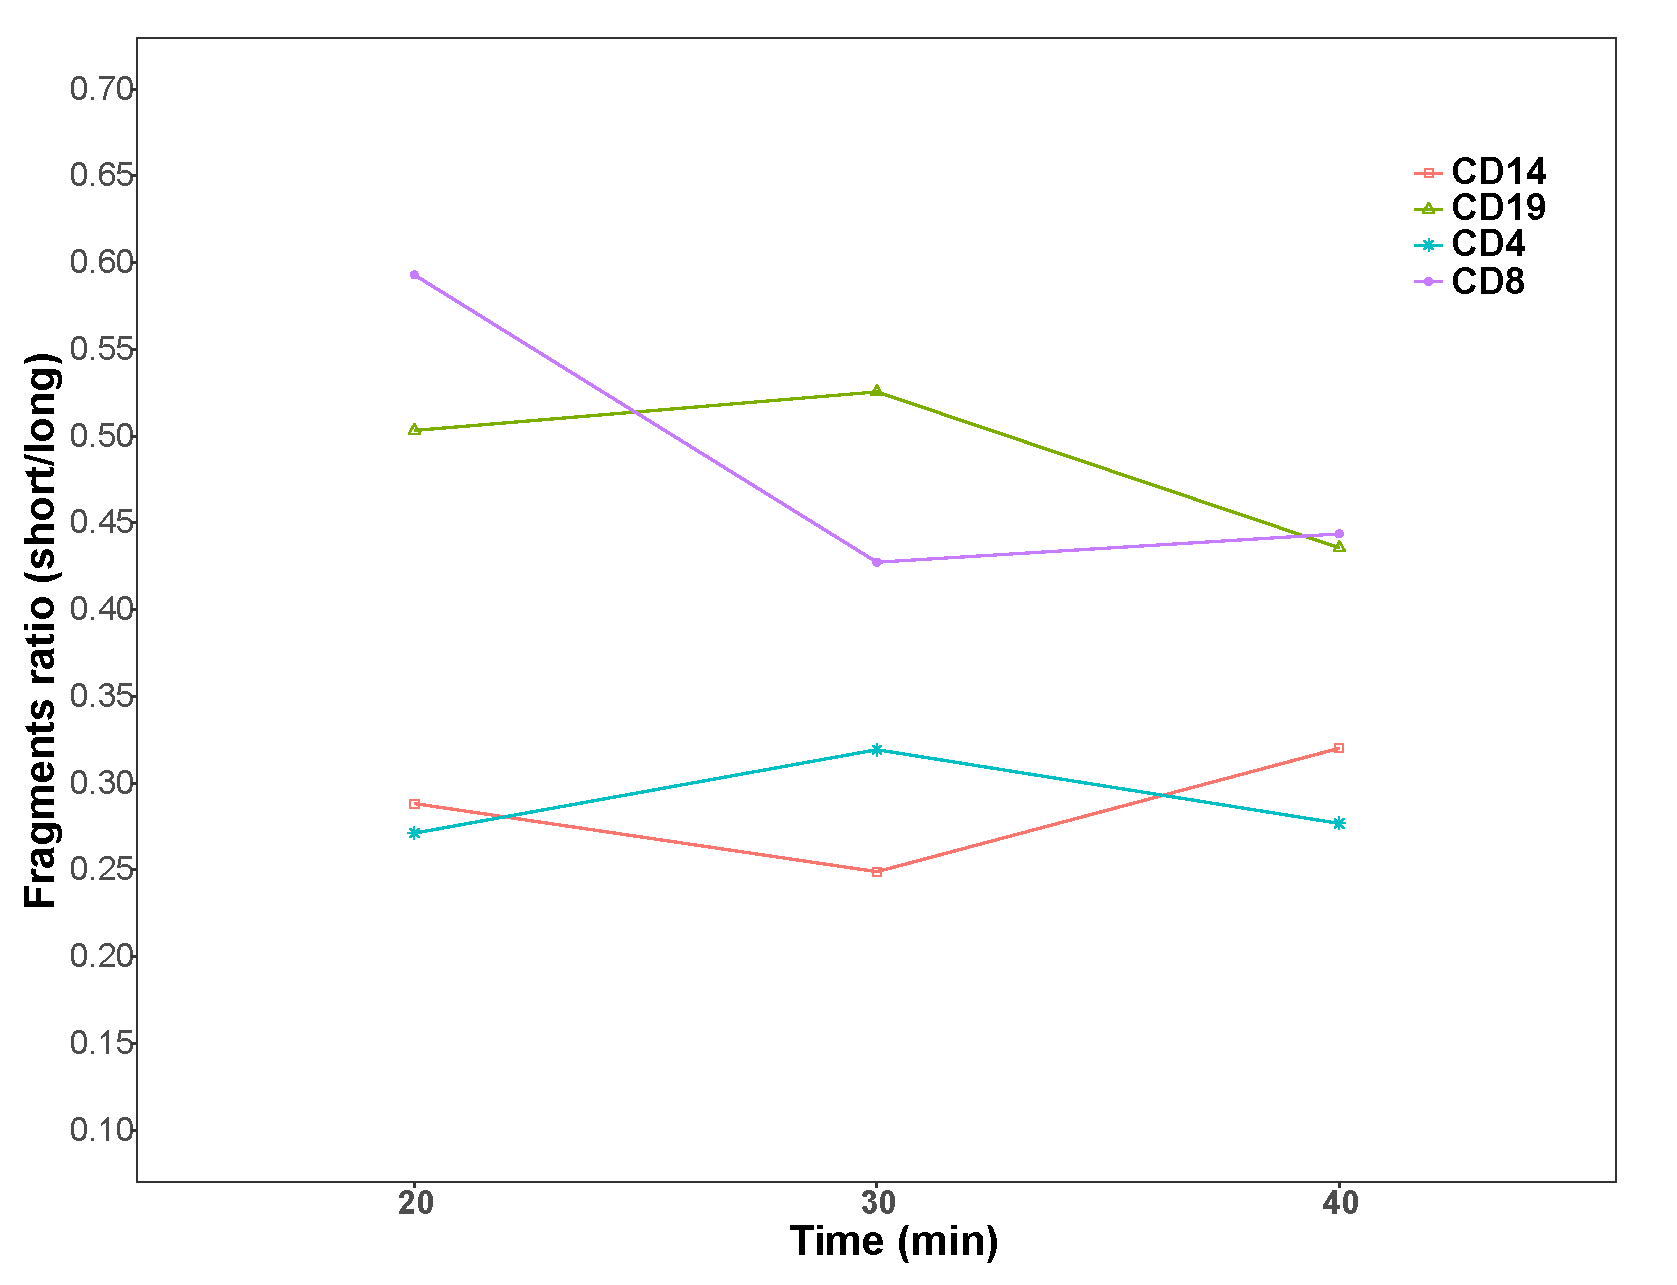
\includegraphics[width=\textwidth]{./Results1/pdfs/ATAC_ratio_short_long_fragments_20_30_40_min}
\caption{\textbf{}}
\end{subfigure} \\
\begin{subfigure}{0.5\textwidth}
\centering
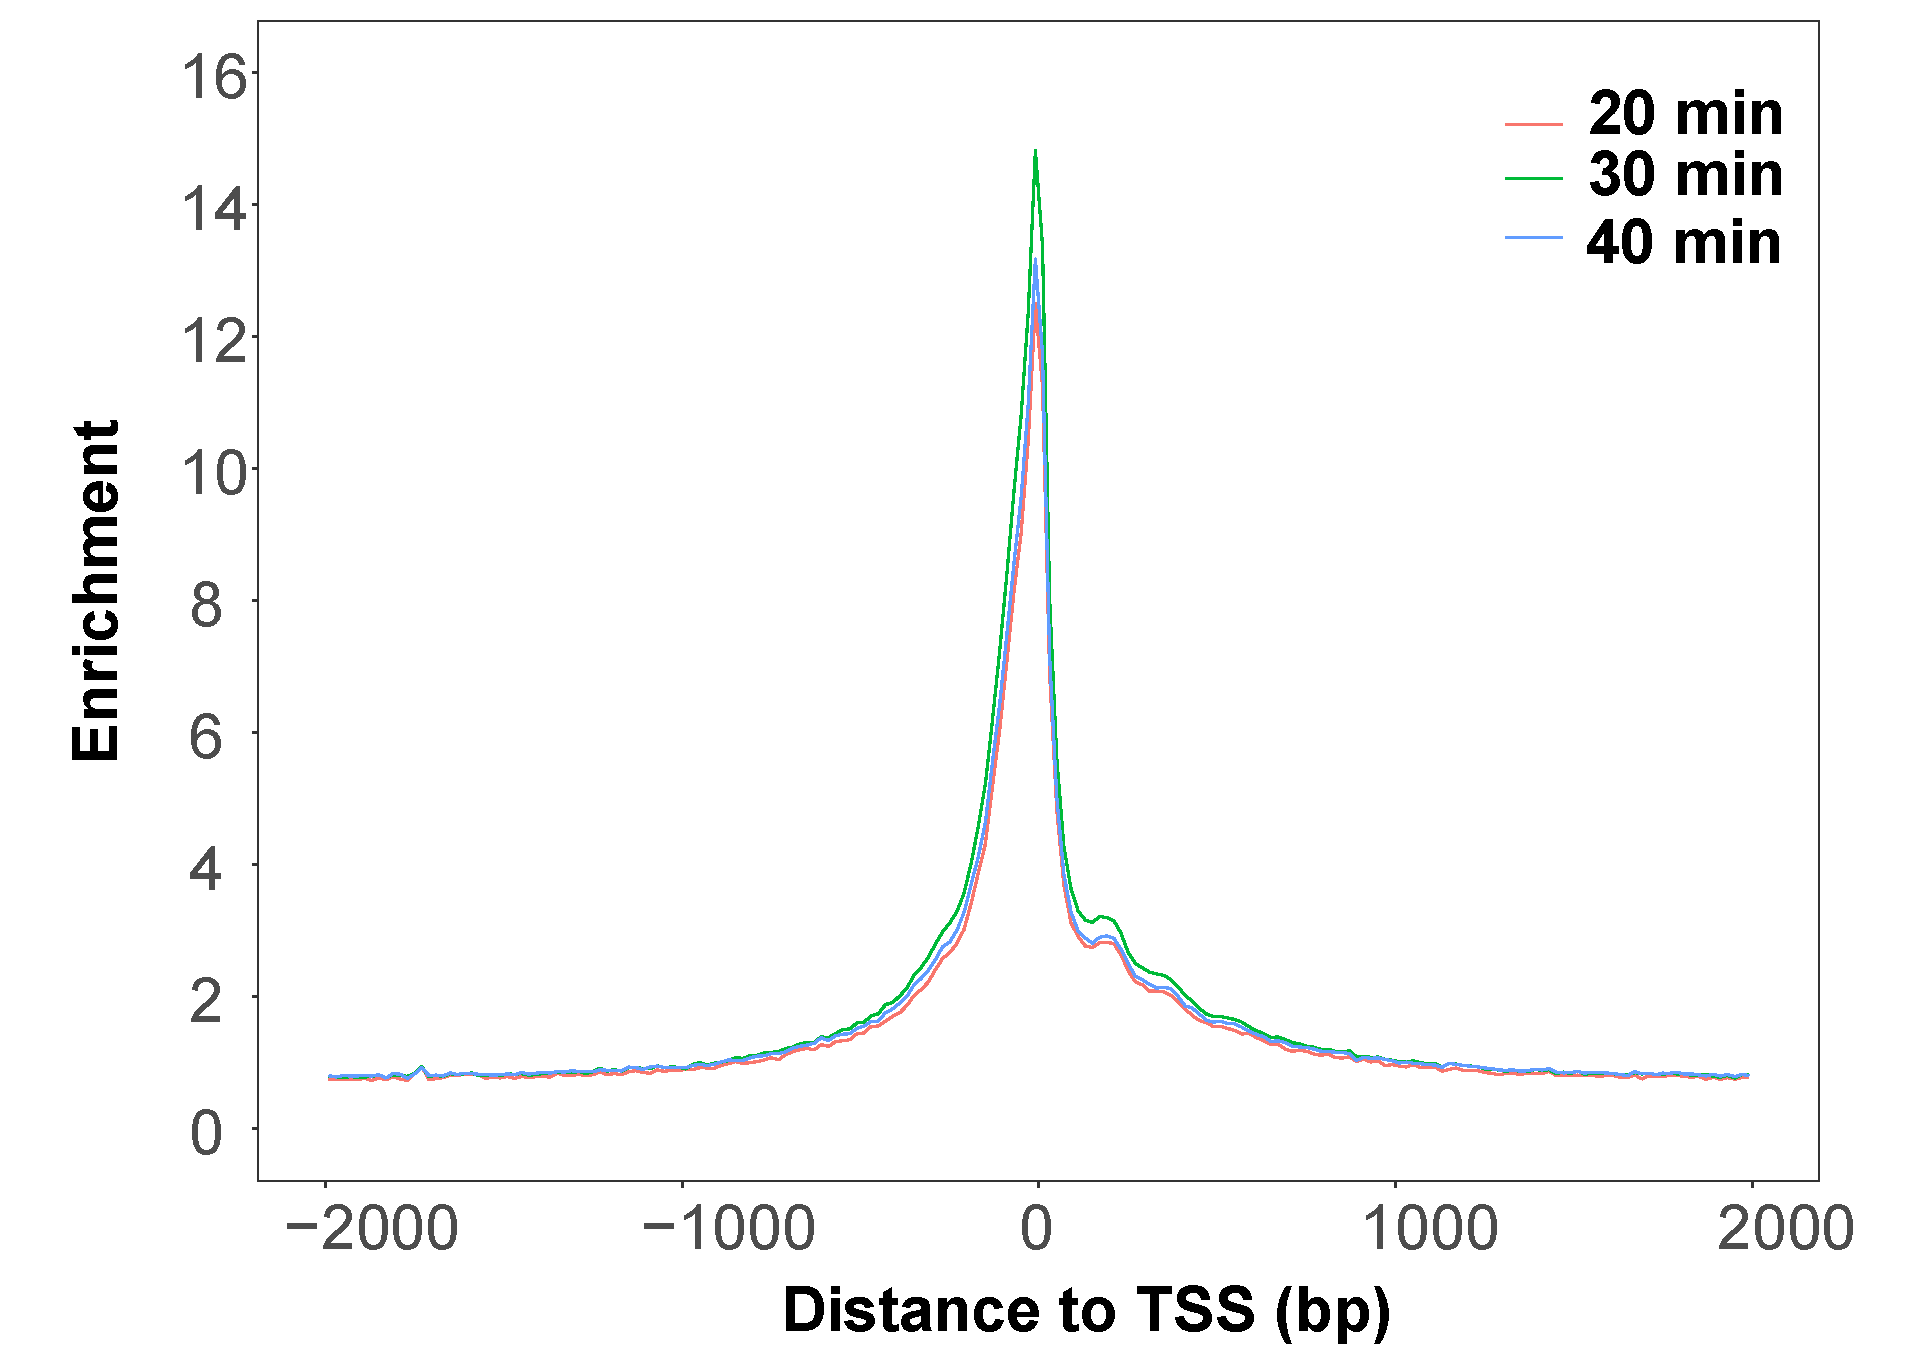
\includegraphics[width=\textwidth]{./Results1/pdfs/ATAC_optimisation_CD4_20_30_40_min_tss_enrichment}
\caption{\textbf{}} % to add text to the figure name
\end{subfigure}
\caption[Assessment of the effect of transposition times on the ATAC-seq QC parameters]{\textbf{Assessment of the effect of transposition times on the ATAC-seq QC parameters} \\
}
\label{fig:Transposition_times_ATAC}
\end{figure} 



\begin{figure}[htbp]
\centering
\begin{subfigure}{0.5\textwidth}
\centering
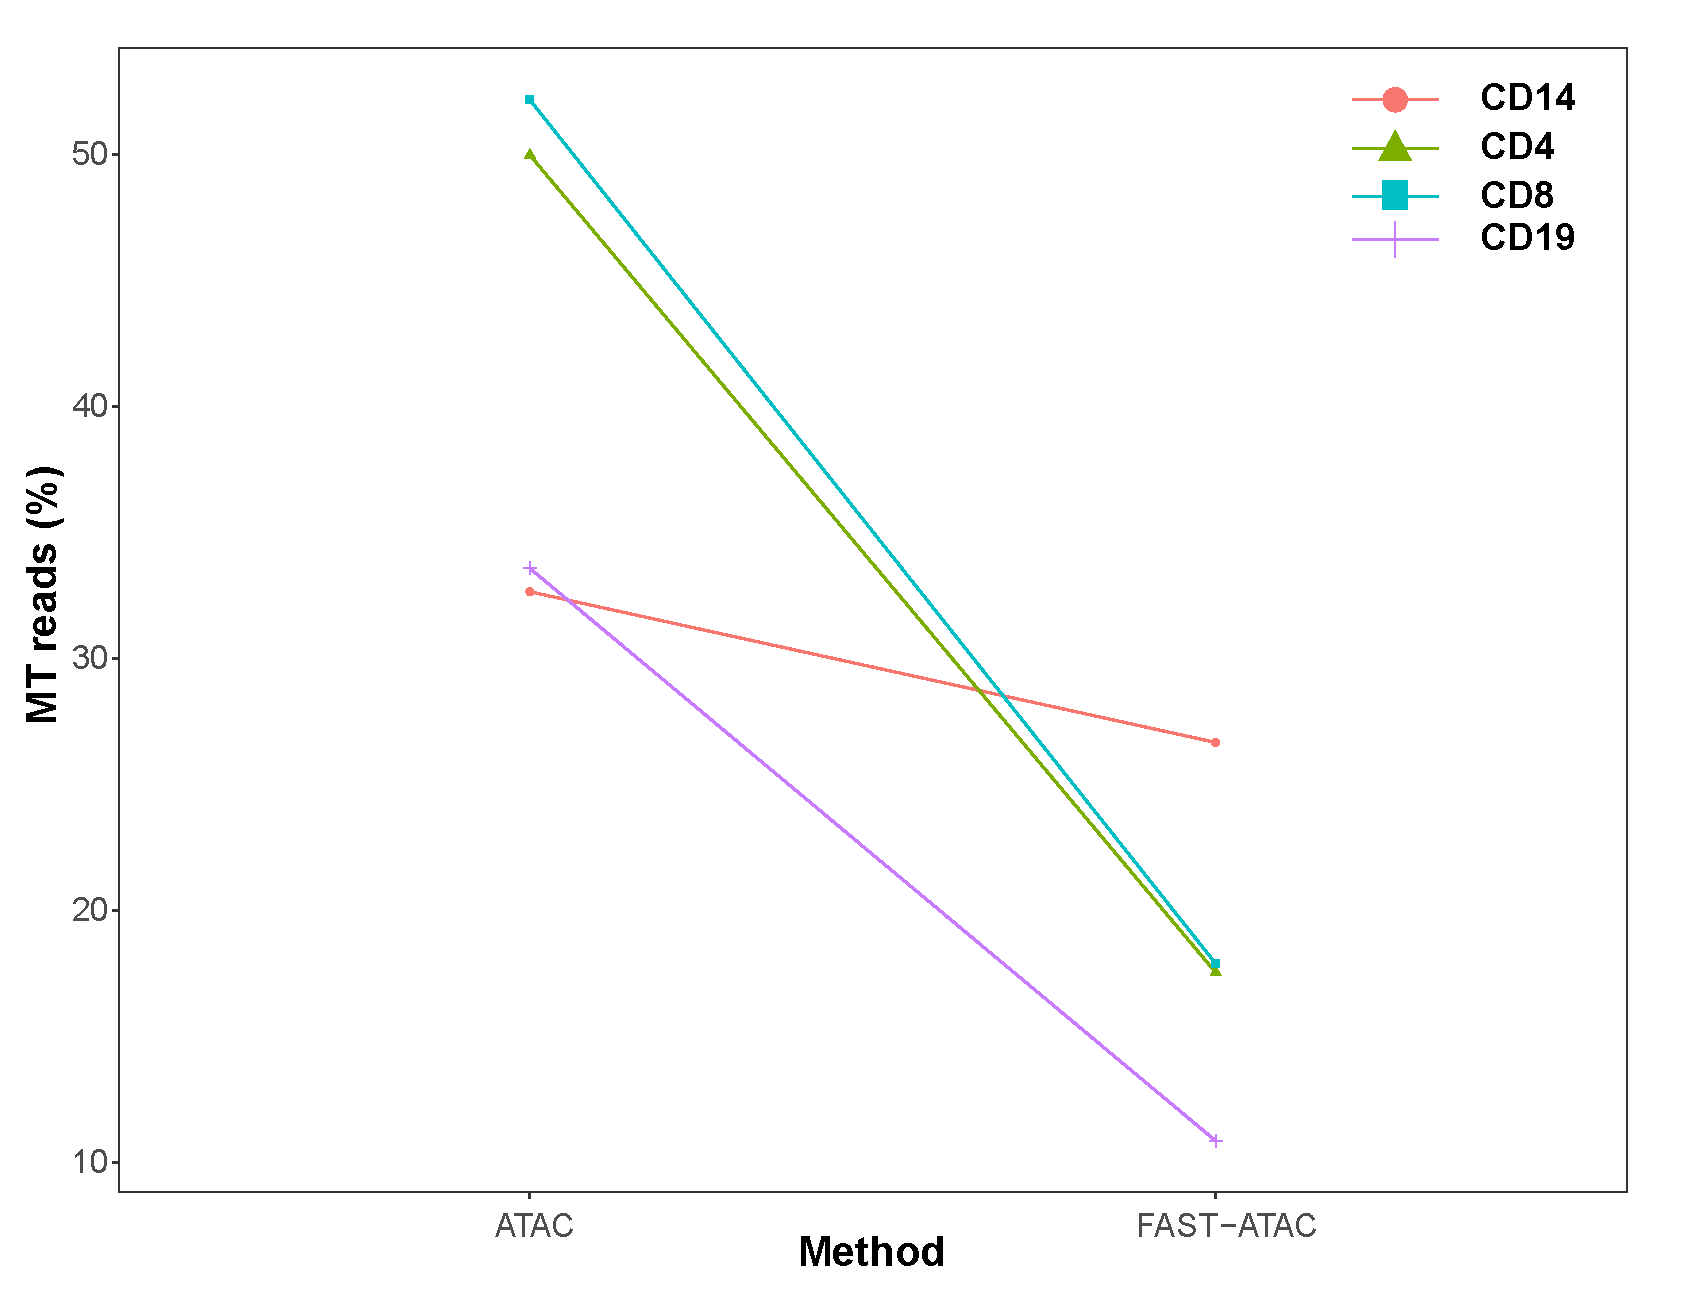
\includegraphics[width=\textwidth]{./Results1/pdfs/ATAC_vs_FAST_ATAC_percnt_MT_reads_dotplot}
\caption{\textbf{}}
% The percentage sign indicated that the other subfig goes side by side
\end{subfigure}%
\begin{subfigure}{0.5\textwidth}
\centering
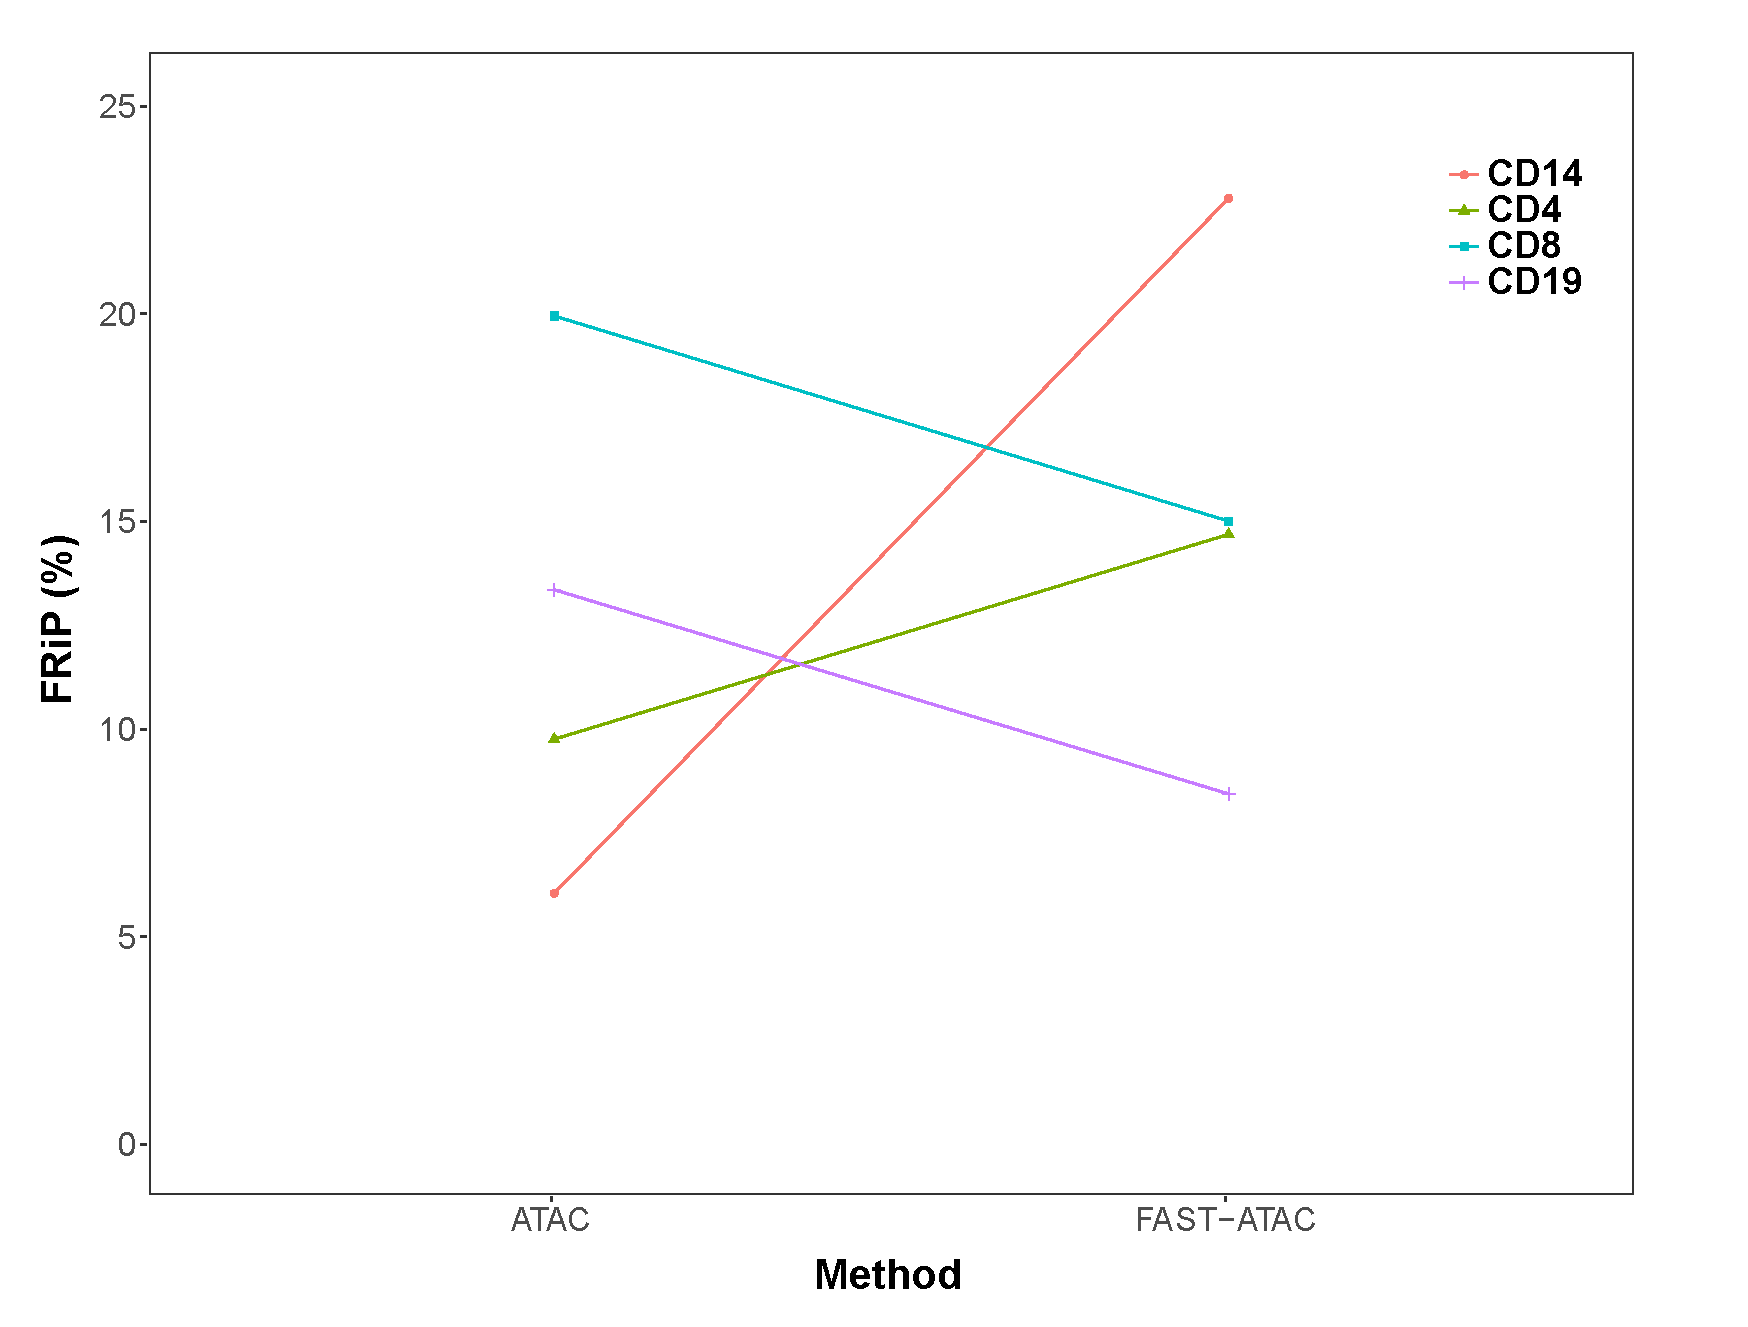
\includegraphics[width=\textwidth]{./Results1/pdfs/ATAC_vs_FAST_ATAC_FRiP_dotplot}
\caption{\textbf{}}
\end{subfigure}
\caption[Differences in MT DNA abundance and signal specificity between ATAC-seq and FAST-ATAC protocols]{\textbf{Differences in MT DNA abundance and signal specificity between ATAC-seq and FAST-ATAC protocols}}
\label{fig:ATAC_vs_FAST_ATAC}
\end{figure} 



\subsection{Limitations of ATAC-seq and FAST-ATAC to assess chromatin accessibility in KC}

Due to the fact that KC is one of the most relevant cell types in psoriasis pathophysiology, ATAC-seq as described in Buenrostro \textit{et al.}, 2013 (named as ATAC-seq 1 here) was performed in 50,000 cells of a suspensions isolated from a psoriasis lesional skin biopsy. Two different tranposition times (30 and 40 min) where tested. Since biopsy handling and lesional epidermal KC are particularly challenging this was considered the best system to test the performance of the standard protocol in the clinical setting of interest for the study. Two tranposition times (30 and 40 min) where tested.


\begin{figure}[htbp]
\centering
\begin{subfigure}{0.45\textwidth}
\centering
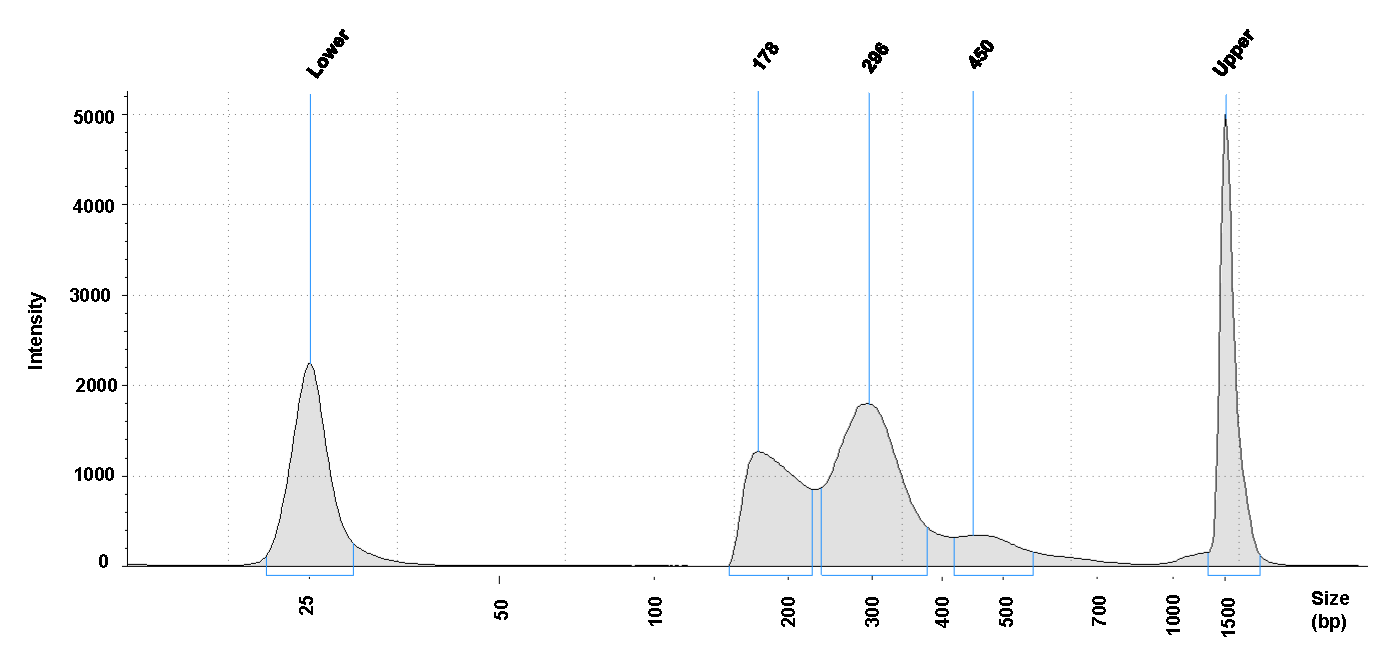
\includegraphics[width=\textwidth]{./Results1/pdfs/ATAC_PS02_tapestation_30min}
\caption{\textbf{}}
% The percentage sign indicated that the other subfig goes side by side
\end{subfigure}
\begin{subfigure}{0.45\textwidth}
\centering
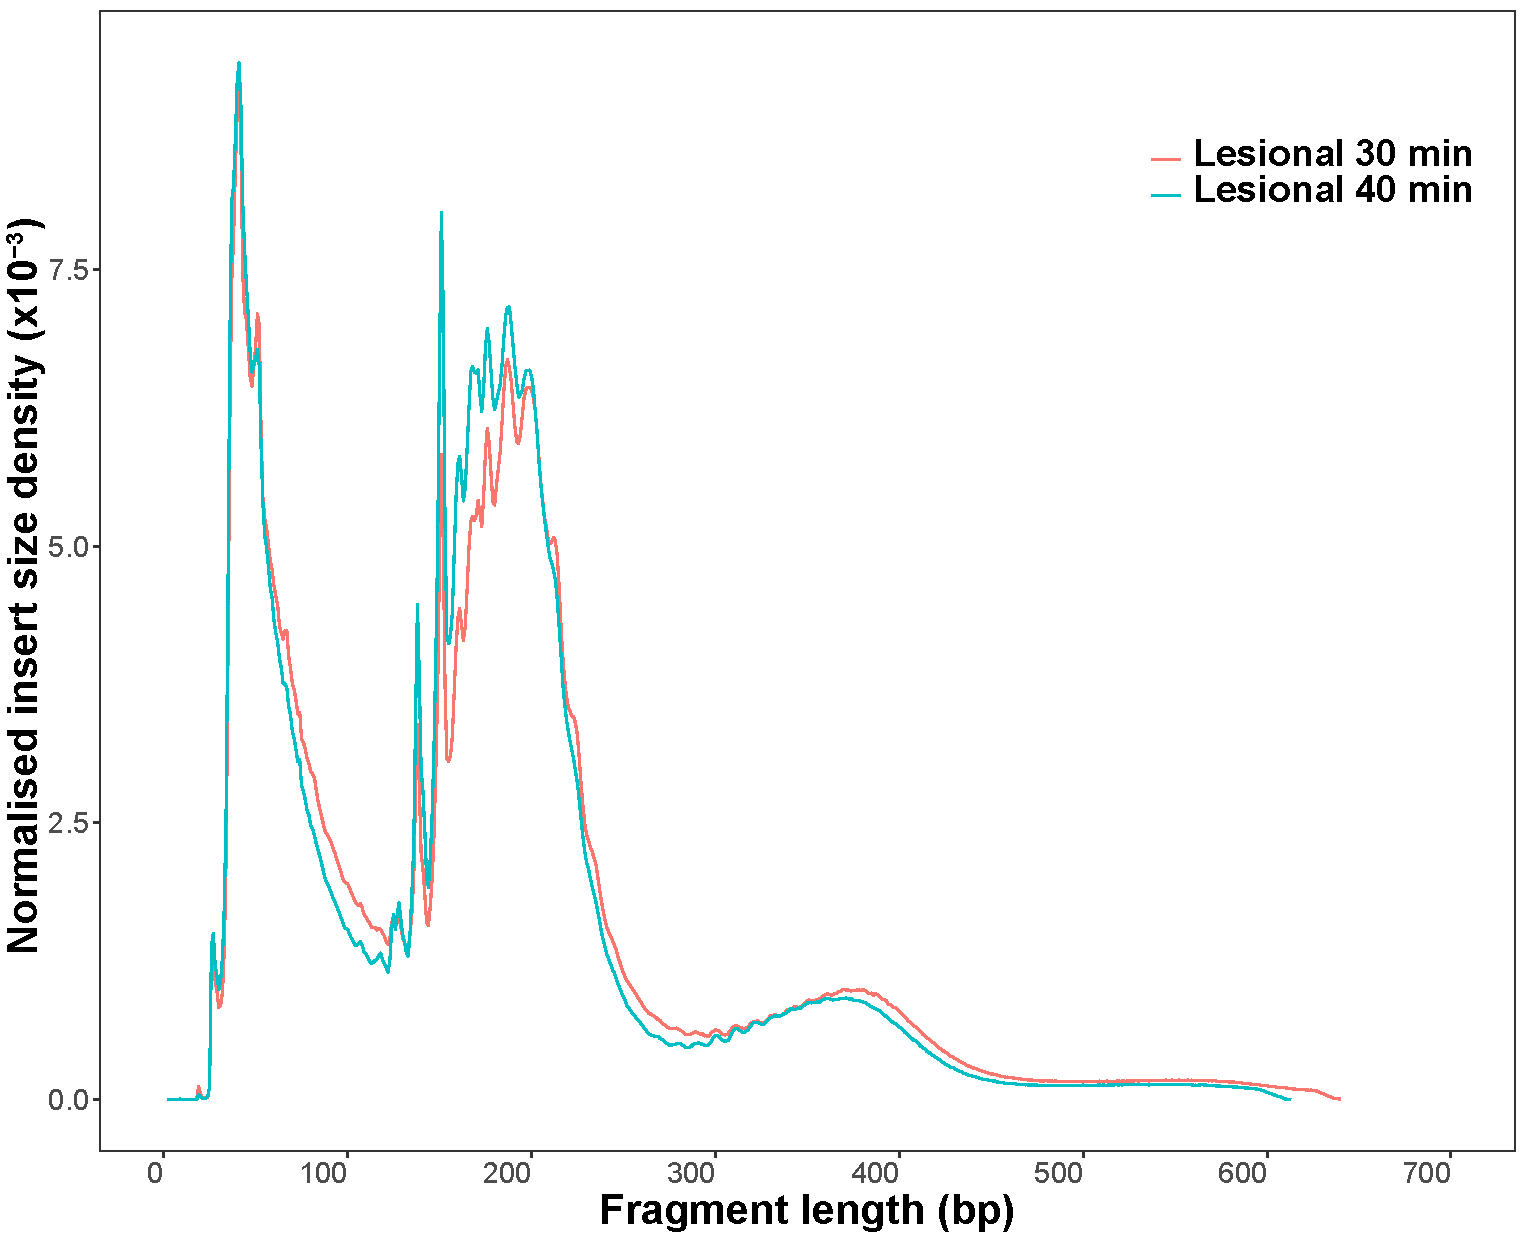
\includegraphics[width=\textwidth]{./Results1/pdfs/ATAC_PS-2_30_40_min_fragment_size_distribution}
\caption{\textbf{}}
\end{subfigure}
\begin{subfigure}{0.5\textwidth}
\centering
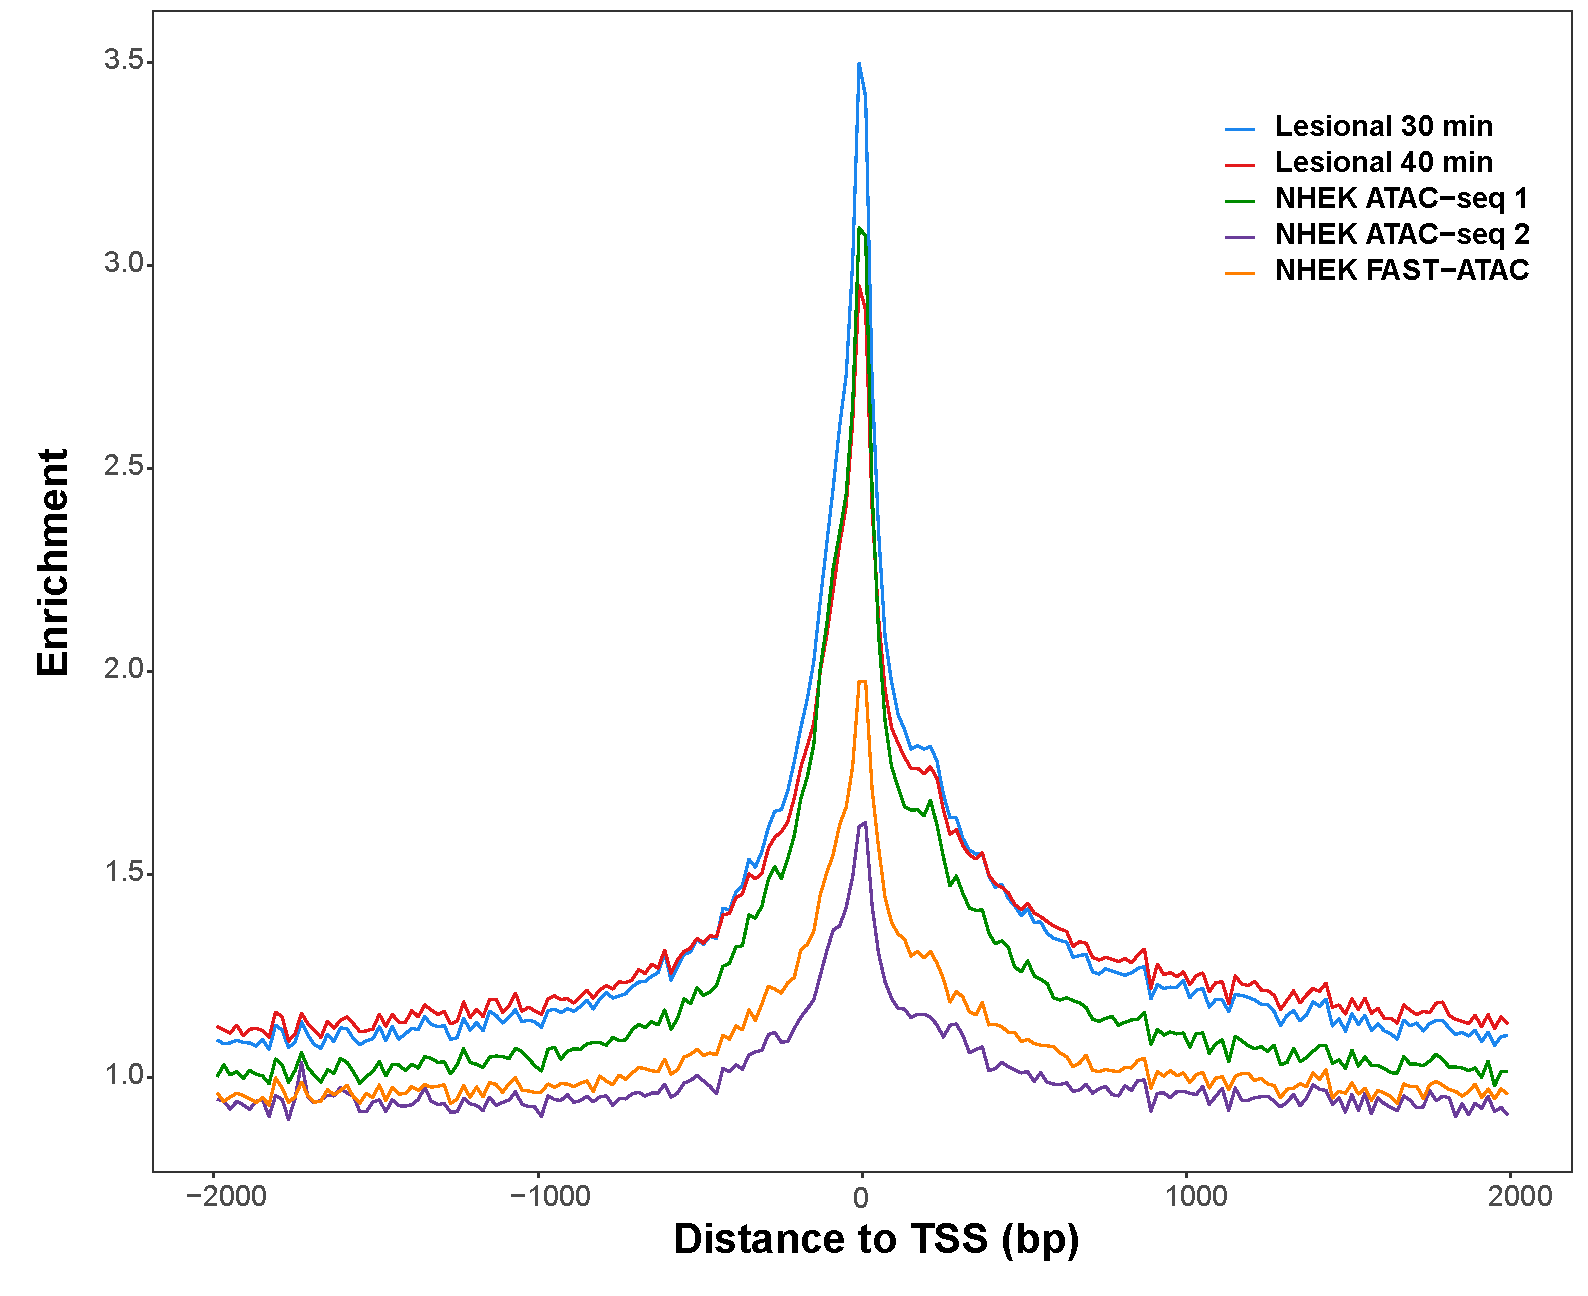
\includegraphics[width=\textwidth]{./Results1/pdfs/ATAC_skin_TSS_enrichment_PS02_30_40min_NHEK_ATAC1_ATAC_2_FAST_ATAC}
\caption{\textbf{}} % to add text to the figure name
\end{subfigure}%
\caption[QC assessment of ATAC-seq in KC enriched cell suspension derived from a psoriatic lesional skin biopsy]{\textbf{QC assessment of ATAC-seq in KC enriched cell suspension derived from a psoriatic lesional skin biopsy}. Two transposition times (30 and 40 min) were tested using the standard ATAC-seq protocol (Buenrostro \textit{et al.}, 2013 in 50,000 cells from the same suspension.}
\label{fig:PS02_skin_ATAC_QC_assessment}
\end{figure} 




Although cell suspension obtained from biopsies using trypsinisation of the epidermal sheet are 90\% enriched in KC, they also contain significant amounts of dead cells and free-DNA releases by apoptotic cells. In order to overcome this problem and the impact that it may have over ATAC-seq background signal, viable KC were selected by adherence assay. Biopsy cell suspensions were cultured for 3h in a 96-well plate and washed afterwards to ensure that only the viable and less differentiated KC would remain for down stream analysis. In parallel cultured NHEK were also used to assess the performance of the different ATAC-seq protocols.

Table for the conditions: done
Tapestation profiles of the the chosen condition. done Send the others to supplementary.
QC measurements: for ATAC1, ATAC2 and NHEK, mention frag size distribution done
DHS enrichment for p and q done but not convincing.The complex network of keratin filaments in stratified epithelia is tightly regulated during squamous cell differentiation. Keratin 14 (K14) is expressed in mitotically active basal layer cells, along with its partner keratin 5 (K5), and their expression is down-regulated as cells differentiate.


\begin{table}[htbp]
\setlength{\tabcolsep}{20pt} only to stretch the columns if you want
\renewcommand{\arraystretch}{1.5}
\begin{tabular}{@{} c c c}
\toprule
\textbf{Protocol} & \textbf{Lysis and} & \textbf{Key parameters} \\
                  & \textbf{transposition} &  \\
\midrule
\midrule
Buenrostro \texit{et al.,} 2013 & Two steps & 0.1\% NP-40 and 2.5$\micro$L Tn5  \\
\midrule
Bao \texit{et al.,} 2015        &Two steps   & 0.05\% NP-40 and 5$\micro$L Tn5  \\
\midrule
                                &          & C1: 0.01\% digitonin, 0.5$\micro$L Tn5 \\
                                &          & C2: 0.01\% digitonin, 2.5$\micro$L Tn5 \\
 Corces \texit{et al.,} 2016    & One step & C3: 0.025\% digitonin, 0.5$\micro$L Tn5 \\
													      &          & C4: 0.025\% digitonin, 2.5 $\micro$L Tn5 \\
\bottomrule
\end{tabular}
\medskip %gap
\caption[Description of the most relevant parameter from the ATAC-seq and FAST-ATAC protocols assayed in NHEK and skin biopsies.]{\textbf{ Description of the most relevant parameter from the ATAC-seq and FAST-ATAC protocols assayed in NHEK and skin biopsies.}Transposition for all the different protocols was 30 min.}
\label{tab:ATAC_skin_optimisation_protocols}
\end{table}
\bigskip %bigger space



\begin{figure}[htbp]
\centering
\begin{subfigure}{0.48\textwidth}
\centering
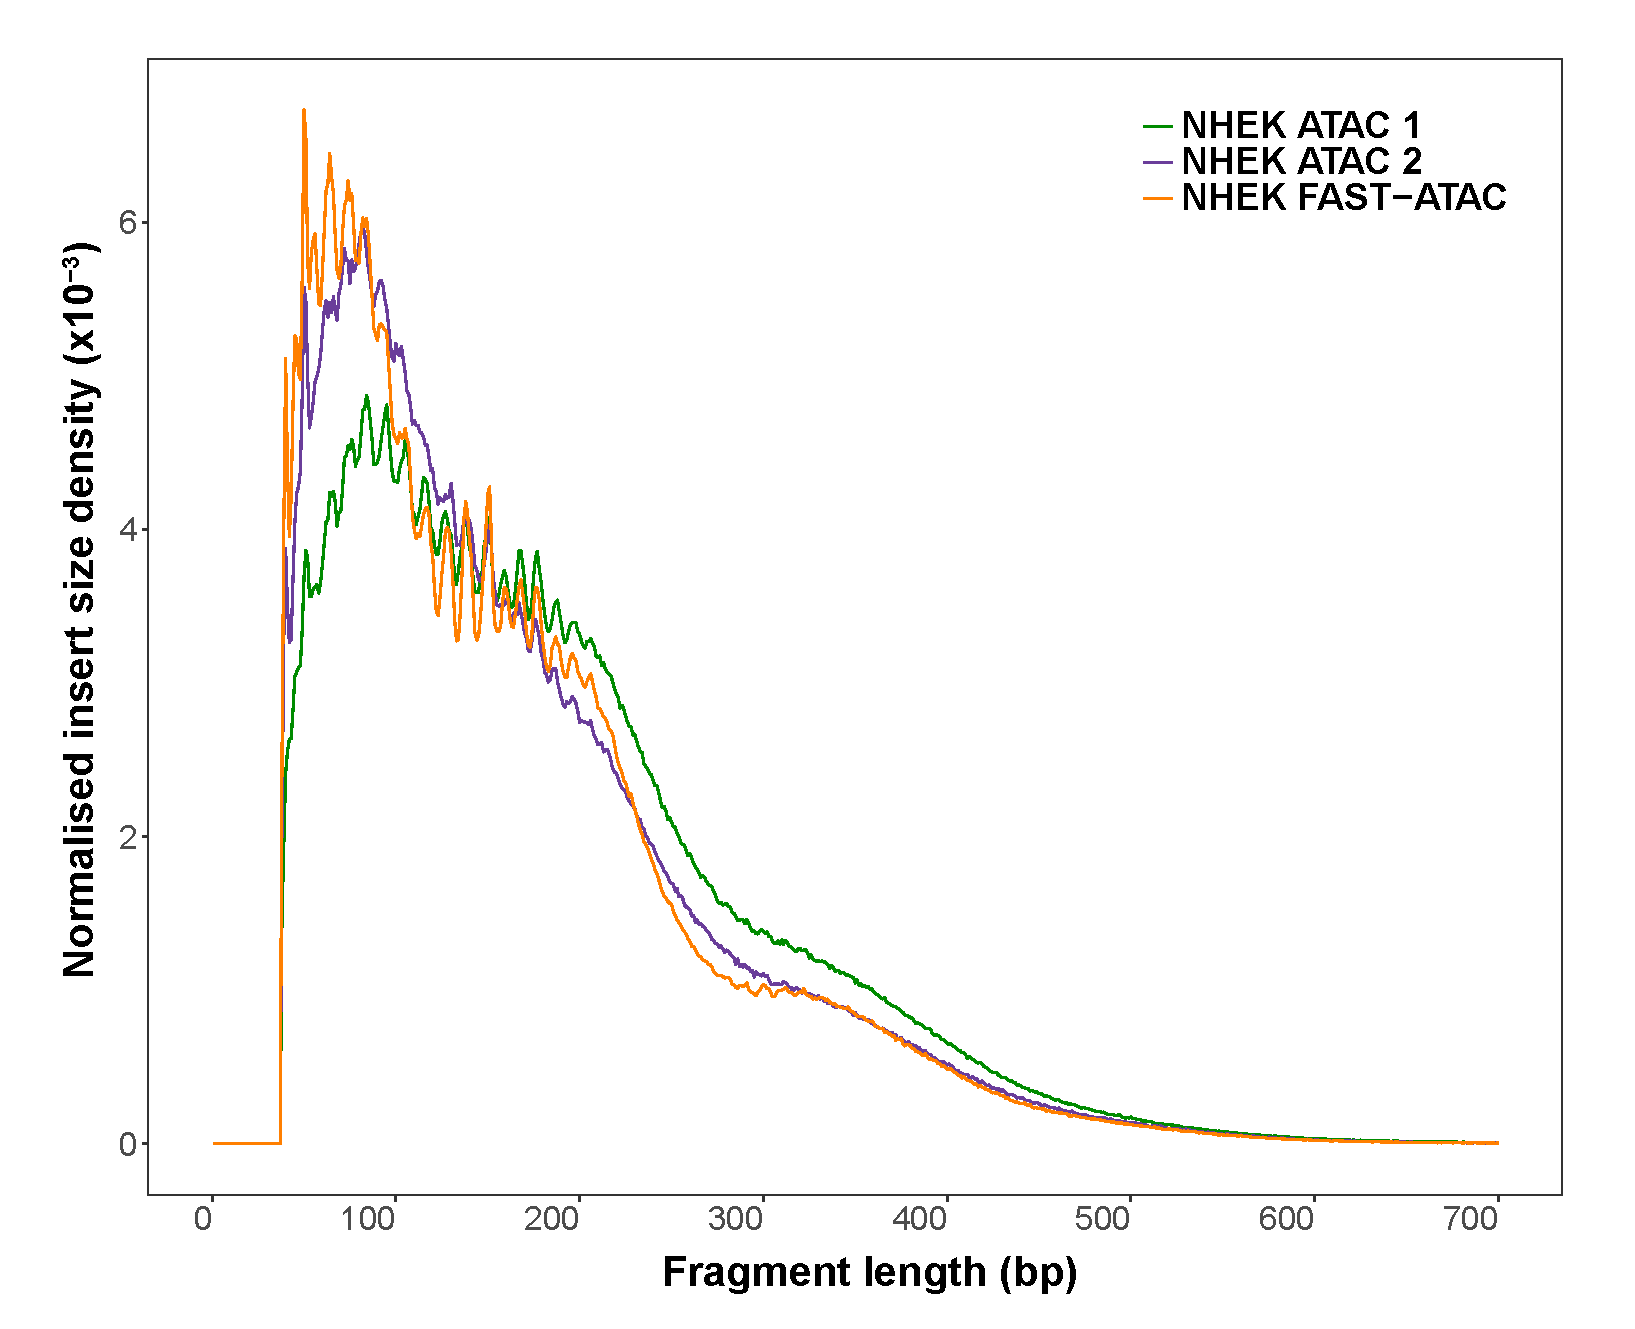
\includegraphics[width=\textwidth]{./Results1/pdfs/ATAC_NHEK_ATAC1_ATAC2_FAST_ATAC_fragment_size_distribution}
\caption{\textbf{}}
\end{subfigure}%
\begin{subfigure}{0.48\textwidth}
\centering
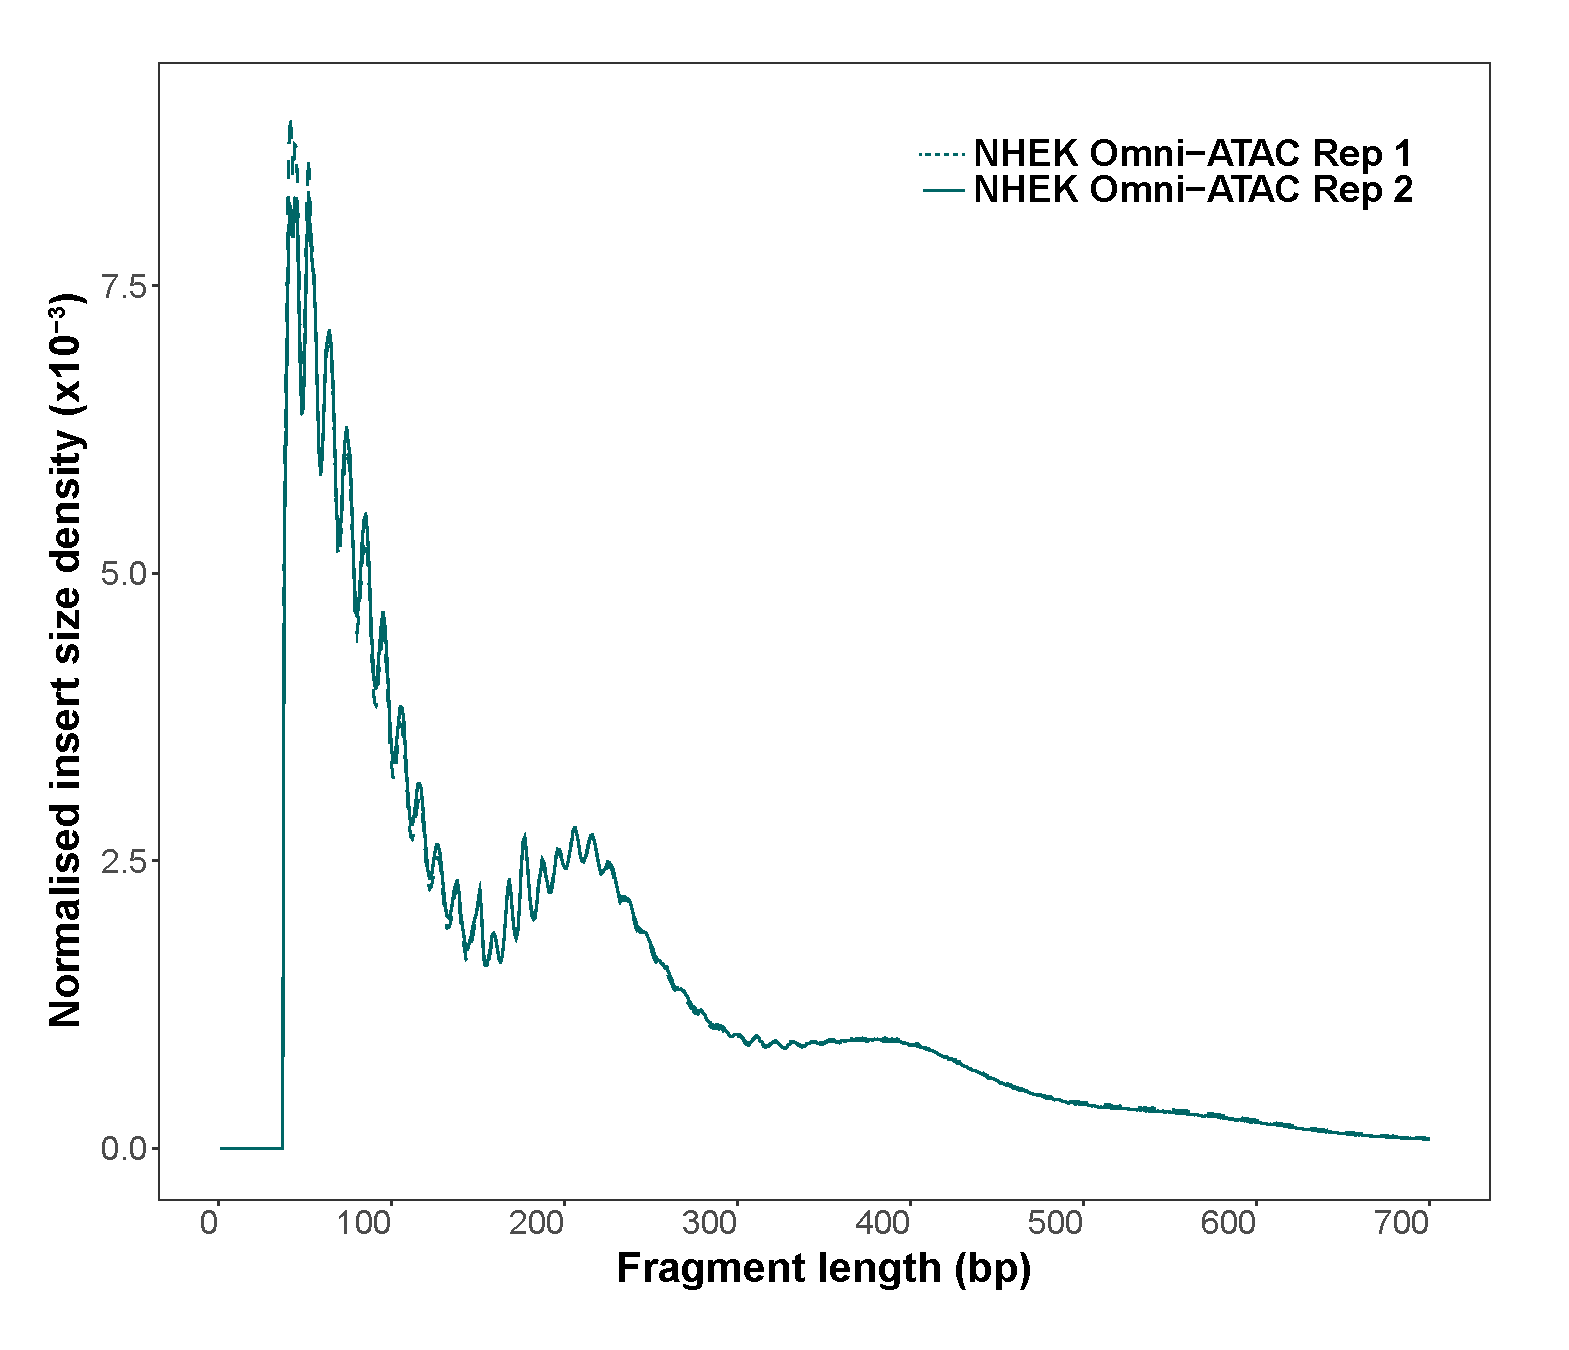
\includegraphics[width=\textwidth]{./Results1/pdfs/ATAC_NHEK_Omni_ATAC_fragment_size_distribution}
\caption{\textbf{}}
\end{subfigure}
\begin{subfigure}{0.5\textwidth}
\centering
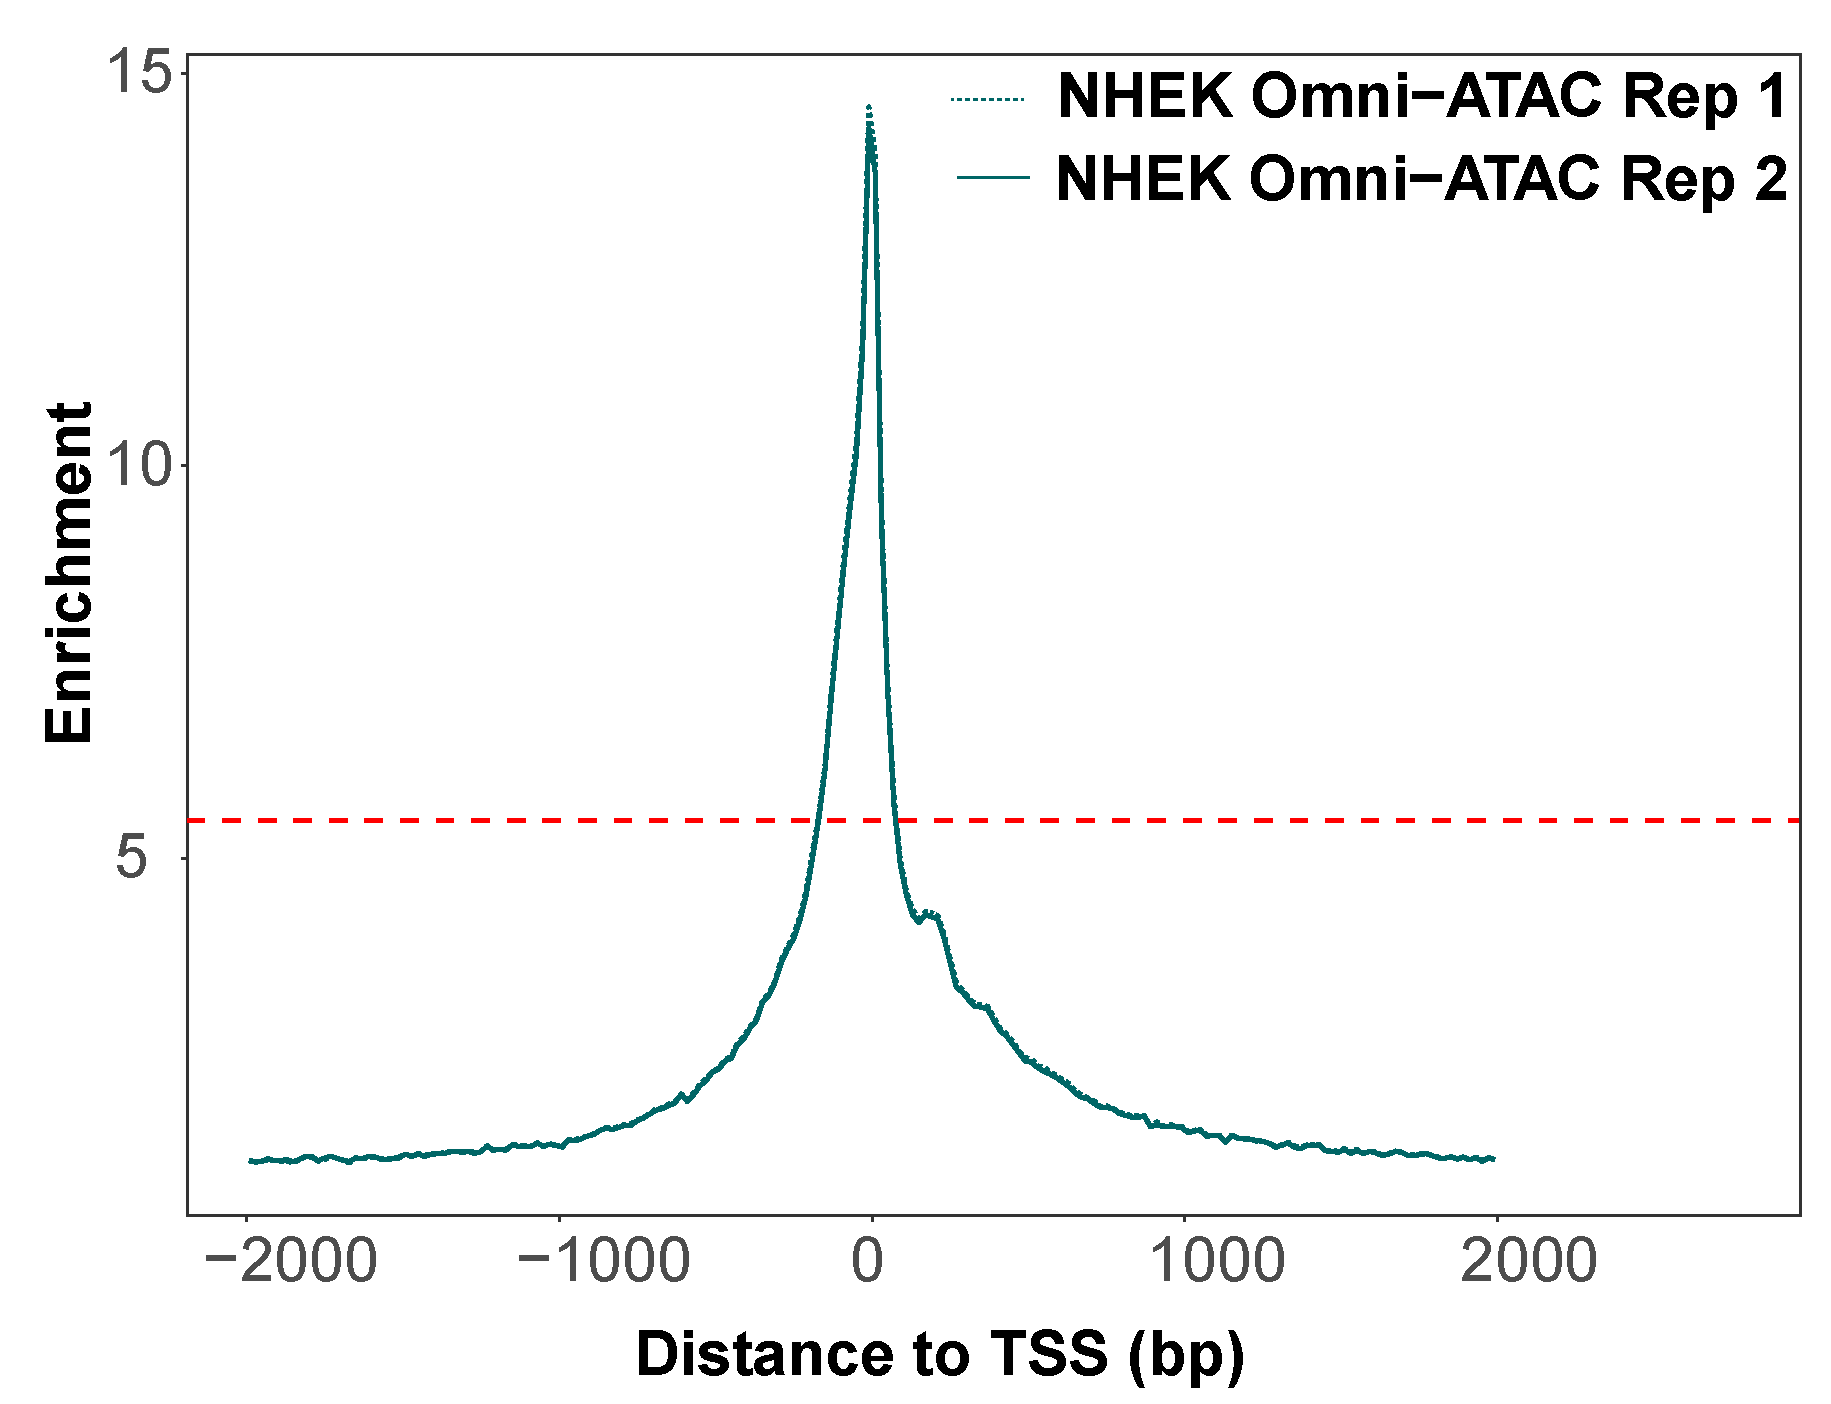
\includegraphics[width=\textwidth]{./Results1/pdfs/ATAC_skin_TSS_enrichment_NHEK_omni_ATAC}
\caption{\textbf{}} % to add text to the figure name
\end{subfigure}%
\caption[QC assessment of FAST-ATAC and Omni-ATAC in cultured NHEK]{\textbf{QC assessment of FAST-ATAC and Omni-ATAC in cultured NHEK.\\
}}
\label{fig:PS02_skin_ATAC_QC_assessment}
\end{figure} 






Omni-ATAC
Tapestation profiles of the the chosen condition include it with the supplementary that includes all other tapestation profiles.done
QC measurements: frag size distribution and TSS done
Track including all skin samples

Think of what to include about the biopsies in supplementary done



\begin{figure}[htbp]
\centering
\begin{subfigure}{0.5\textwidth}
\centering
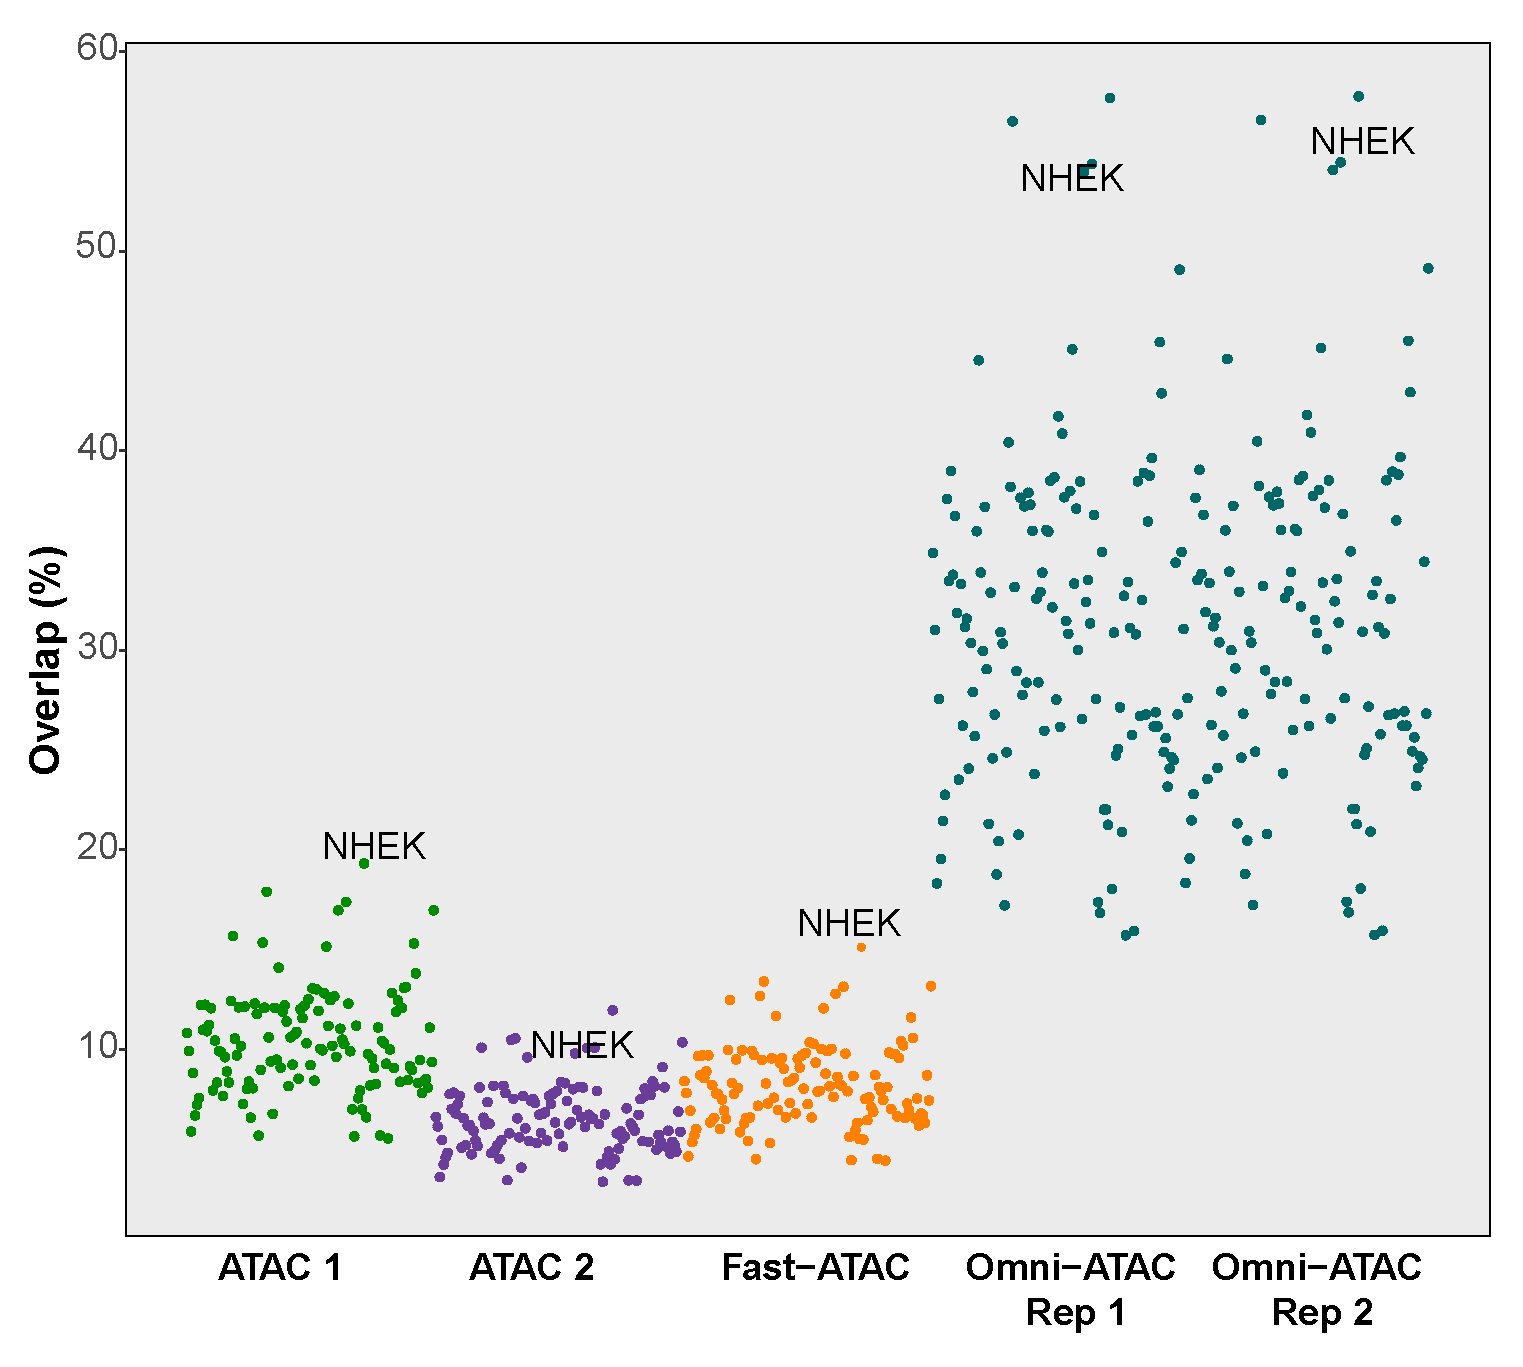
\includegraphics[width=\textwidth]{./Results1/pdfs/ENCODE_125_cell_types_overlap_FAST_ATAC_Omni_ATAC_pval_2}
\caption{\textbf{}}
% The percentage sign indicated that the other subfig goes side by side
\end{subfigure}%
\begin{subfigure}{0.5\textwidth}
\centering
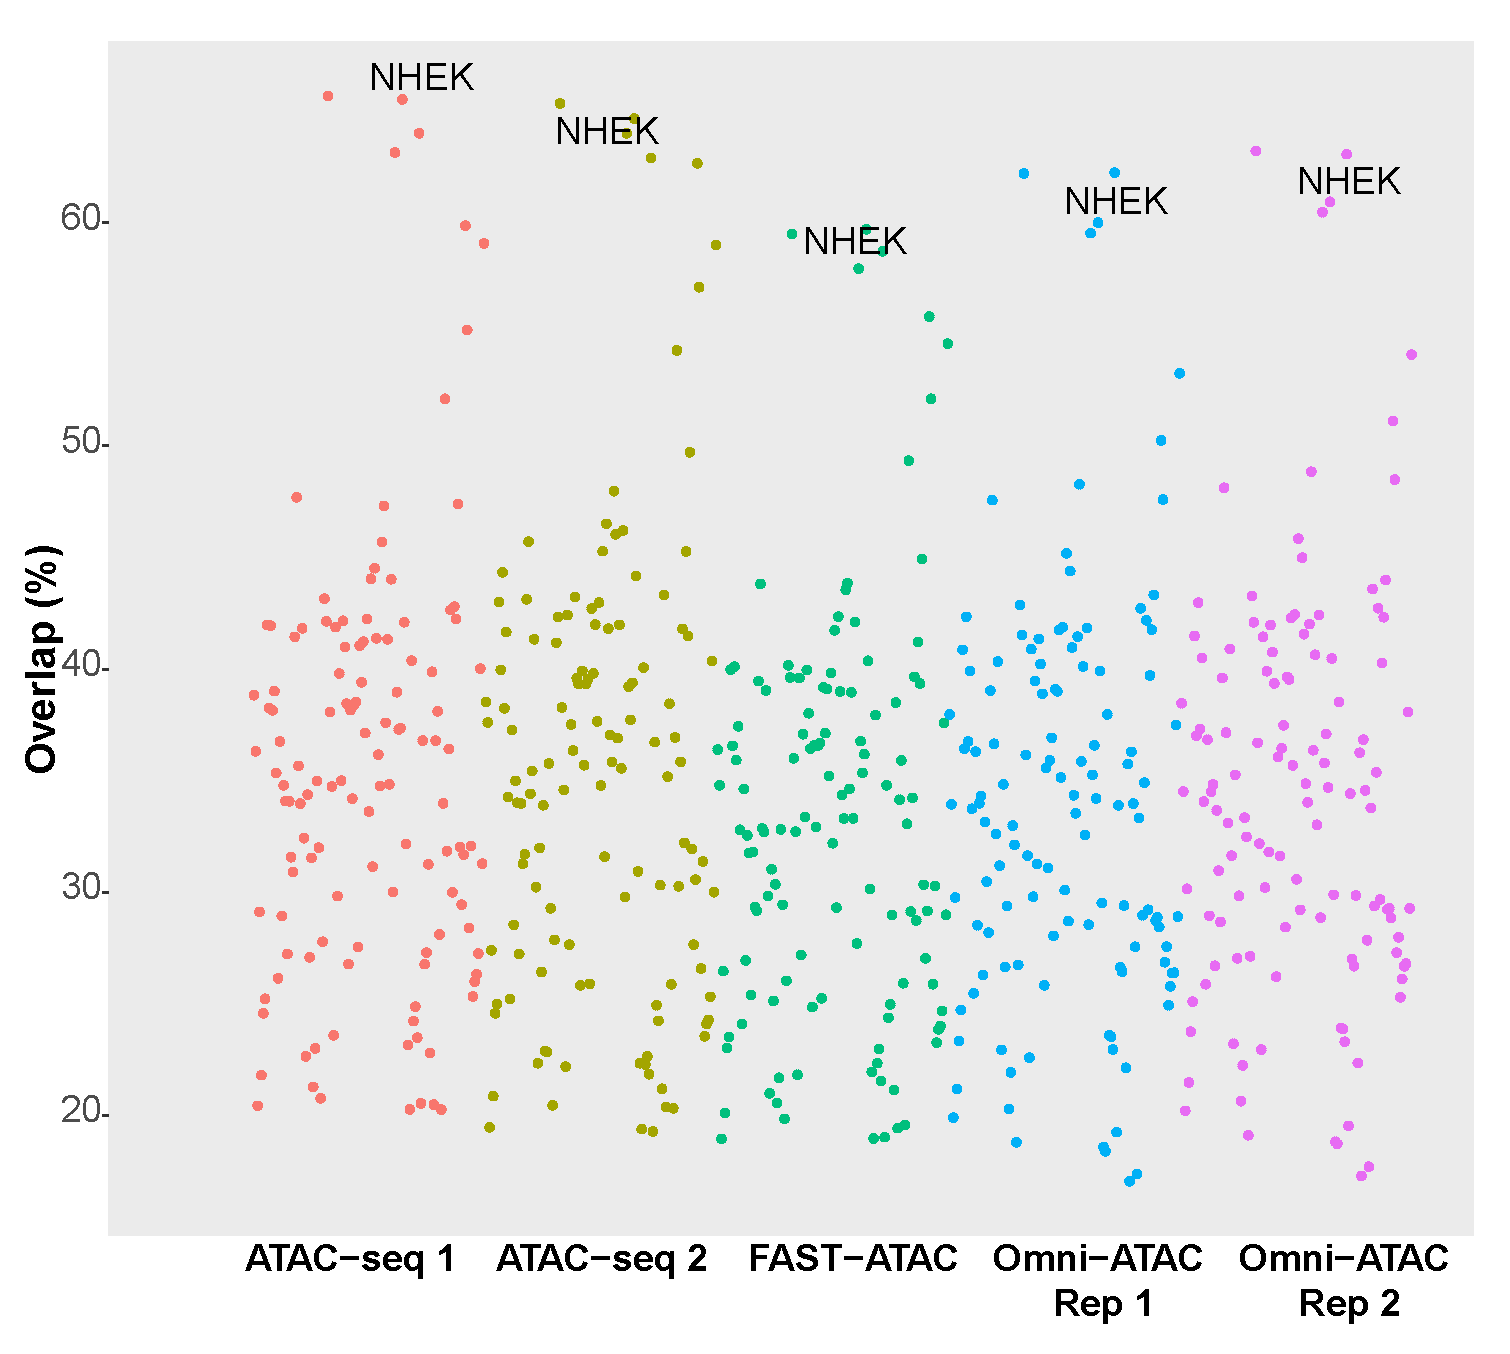
\includegraphics[width=\textwidth]{./Results1/pdfs/ENCODE_125_cell_types_overlap_FAST_ATAC_Omni_ATAC_qval_2}
\caption{\textbf{}}
\end{subfigure}
\begin{subfigure}{0.5\textwidth}
\centering
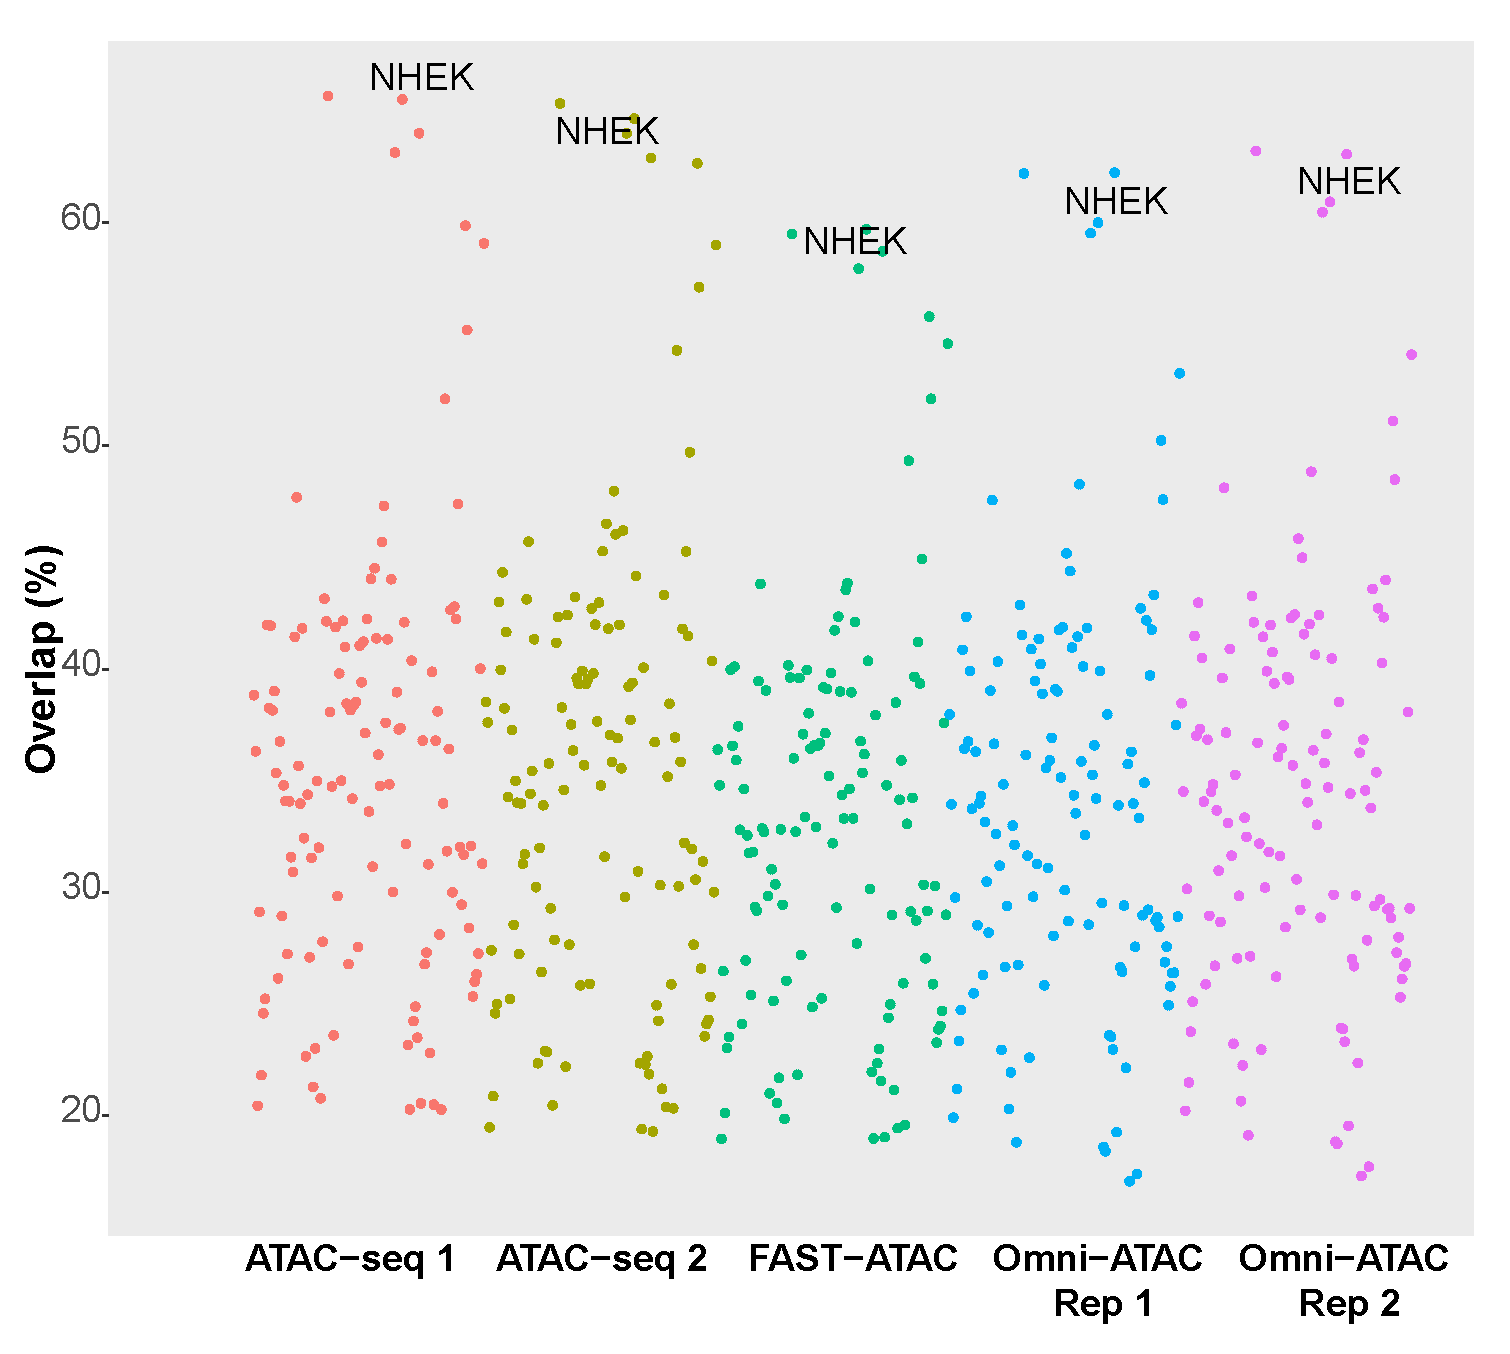
\includegraphics[width=\textwidth]{./Results1/pdfs/ENCODE_125_cell_types_overlap_FAST_ATAC_Omni_ATAC_qval_2}
\caption{\textbf{}} % to add text to the figure name
\end{subfigure}%
\caption[QC assessment of Omni-ATAC in NHEK and chromatin accessibility signal for the samples generated with the different ATAC-seq protocols]{\textbf{QC assessment of Omni-ATAC in NHEK and chromatin accessibility signal for the samples generated with the different ATAC-seq protocols}.\\}
\label{fig:Omni_ATAC_NHEK_QC_assessment_and_all_tracks}
\end{figure} 
